\documentclass[pregrado]{tesis-usb}

% paquetes
\usepackage[utf8]{inputenc}
\usepackage{verbatim}
\usepackage{acronym}
\usepackage{amsmath}
\usepackage{amsfonts}
\usepackage{amssymb}
% \usepackage{hyperref}

% estilo de las referencias
\usepackage[fixlanguage]{babelbib-and}\selectbiblanguage{spanish}
\usepackage{url}
\bibliographystyle{babplain-lf}

\autor{Esteban de Jesús Rafael Camargo Rodríguez}
\usbid{11-10145}
\titulo{Diseño de simulador de hornos de proceso}
\tutor{Antonio Cavero}
\usarcotutor
\cotutor{Euler Jimenez} 
\trabajo{Proyecto de grado}
\coord{Ingeniería Química}
\grado{Ingeniero Químico}
\fecha{Mayo~de~2022}

\autori{E. Camargo}
\agno{2022}
\fechadefensa{30~de~Mayo~de~2022}
\carrera{Ing. Química}

\programa{Nombre del Programa}
\juradouno{Alejandro Requena}
\juradodos{Sabrina D'Scipio \mbox{(Afiliaci\'on)}}
\juradotres{Claudio Olivares}

% Cambia comillas simple por comilla cerrada en ambiente verbatim 
\makeatletter
\let \@sverbatim \@verbatim
\def \@verbatim {\@sverbatim \verbatimplus}
{\catcode`'=13 \gdef \verbatimplus{\catcode`'=13 \chardef '=13 }} 
\makeatother

\begin{document}

\frontmatter
\maketitle
\chapter*{Dedicatoria}

\par Dedicado a la Universidad Sim\'on Bol\'ivar y a su comunidad.
\par A mis padres.

\chapter*{Agradecimientos}

Gracias a mis tutores, Euler y Antonio, por su gu\'ia en este trabajo, respondiendo atentamente a todas mis preguntas, por su paciencia corrigiendo mis errores y por su constante motivación.\\

Gracias a mi madre, Marlene, por apoyarme incondicionalmente y siempre haber creído en mí.
\begin{resumen}
     El conocimiento al operar un equipo en cualquier planta de ingeniería siempre ha sido algo fundamental, pero hay ocaciones en que el conocimiento práctico se queda corto y no basta con saber manipularlo físicamente, si no también conocer los principios fundamentales detrás del funcionamiento del equipo. Los hornos de procesos en refinerías industriales son equipos asociados al corazón del proceso, y por tanto, requieren de fuertes bases para su correcta manipulación. Teniendo esto en cuenta se diseño este proyecto para generar una aplicación capaz de transmitir de manera eficiente los principios y consecuencias de la manipulación del horno de procesos. El objetivo de la herramienta es encargarse de simular las posibles interacciones de un operador con el equipo, con su uso los operadores podrán tener una idea de como cambiará el proceso dependiendo de las variables que decidan alterar, las cuales pueden ser el flujo del crudo, la apertura o cierre de los ductos de alimentación de aire o salida de gases de chimenea y por último la cantidad de combustible suministrado al horno. \\
     
     Palabras claves: Fire heater, Horno, Intercambiador, Simulador.
\end{resumen}
\tableofcontents
\listoffigures
\listoftables
\useacronyms
\chapter*{Lista de símbolos}
\begin{tabular}{ll}

$AC_{masa}$ & Relación aire/combustible másica [-] \\
$AC_{molar}$& Relación aire/combustible molar [-] \\
$Afo$   & Área de superficie externa de aletas [m$^2$] \\
$Apo$   & Área de superficie expuesta de tubos lisos [m$^2$] \\
$A_0$   & Área de superficie externa total [m$^2$] \\
$At$    & Área externa del banco de tubos por zona del horno [m$^2$] \\
$Acp$   & Área de plano equivalente por zona del horno [m$^2$] \\
\\
$C_{1,3,5}$ & Coeficientes del factor de Colburn \\
$C_p$   & Calor específico [kJ/kg-K] \\
$C_{p_a}$   & Calor específico del aire [kJ/kg-K] \\
$C_{p_c}$   & Calor específico del combustible [kJ/kg-K] \\
$C_{p_f}$   & Calor específico del fluido [kJ/kg-K] \\
$C_{p_g}$   & Calor específico de los gases de combustión [kJ/kg-K] \\

$d_f$ & Diámetro externo de la aleta [m] \\
$d_o$ & Diámetro externo del tubo [m] \\

$E$   & Eficiencia de las aletas [-]\\
$F$   & Factor global de transferencia radiante [-]\\
$G$   & Velocidad másica basada en el área interna de tubos radiantes [kg/h-m$^2$]\\
$G_n$ & Velocidad másica basada en el área libre para el flujo de gas [kg/h-m$^2$]\\
\\
$h_{c}$ & Coeficiente de transferencia de calor convectivo [W/m$^2$-K]\\
$h_{e}$ & Coeficiente de transferencia de calor externo [W/m$^2$-K]\\
$h_{ee}$& Coeficiente de transferencia de calor externo efectivo [W/m$^2$-K]\\
$h_{i}$ & Coeficiente de transferencia de calor interno [W/m$^2$-K]\\
$h_{r}$ & Coeficiente de transferencia de calor radiante [W/m$^2$-K]\\
\\
$j$     & Factor de Colburn [-] \\
$k_f$   & Conductividad térmica del fluido [W/m-K] \\
$k_g$   & Conductividad térmica de los gases de combustión [W/m-K] \\
\\
$\dot m_a$  & Flujo másico de aire [kg/h] \\
$\dot m_c$  & Flujo másico de combustible [kg/h] \\
$\dot m_f$  & Flujo másico de residuo de vacío [kg/h] \\
$\dot m_g$  & Flujo másico de los gases de combustión [kg/h] \\
\end{tabular}

\begin{tabular}{ll}
\\
\\
$n_a$  & Número de moles del aire [mol] \\
$n_c$  & Número de moles del combustible [mol] \\
\\
$l_f$   & Altura de aleta [m] \\
$L_{tubo}$ & Largo efectivo del tubo [m] \\
$N_r$   & Numero de tubos por fila [-] \\
$N_{tubo}$ & Número de tubos por sección [-] \\
\\
$PL$    & \multirow{2}{26em}{Multiplicación de las presiones parciales de CO$_2$ y H$_2$O por MBL [atm-ft]} \\
\\
$PM_a$    & Peso molecular del aire [kg/kmol]\\
$PM_c$    & Peso molecular del combustible [kg/kmol]\\
\\
$P_l$   & Paso de tubo longitudinal [-]\\
$P_t$   & Paso de tubo transversal [-]\\
\\
$Pr$    & Número de Prandtl [-]\\
\\
$Q_{a}$    & Calor sensible del aire [MW] \\
$Q_{absorbido}$ & Calor absorbido por el fluido en el horno [MW] \\
$Q_{c}$    & Calor sensible del combustible [MW] \\
$Q_{conv}$ & Calor transferido por convección [MW] \\
$Q_{CONV}$ & Calor cedido al fluido en la sección convectiva [MW] \\
$Q_{ESC}$ & Calor cedido al fluido en la sección escudo [MW] \\
$Q_{f_e}$ & Calor del fluido entrando [MW] \\
$Q_{f_s}$ & Calor del fluido saliendo [MW] \\
$Q_{g}$   & Calor sensible de los gases de combustión [MW] \\
$Q_{perdidas}$  & Pérdidas de calor al ambiente [MW] \\
$Q_{rad}$ & Calor transferido por radiación [MW] \\
$Q_{RAD}$ & Calor cedido al fluido en la sección radiante [MW] \\
$Q_{radEsc}$& Calor de radiación que pasa a la sección escudo [MW] \\
$Q_{suministrado}$ & Calor suministrado por combustión [MW] \\
\\
$q_{rad}$ & \multirow{2}{26em}{Flujo de calor por unidad de área exterior del tubo en zona radiante [MW/m$^2$]} \\
\\
$Re$    & Número de Reynolds [-]\\
\\
$R_{fi}$  & Factor de ensuciamiento interno de los tubos [m$^2$-K/W] \\
$R_{fe}$  & Factor de ensuciamiento externo de los tubos [m$^2$-K/W] \\
\end{tabular}

\begin{tabular}{ll}
\\
\\
$R_{int}$  & Resistencia convectiva interna [m$^2$-K/W]\\
$R_{ext}$  & Resistencia convectiva externa [m$^2$-K/W] \\
$R_{tube}$ & Resistencia conductiva del tubo [m$^2$-K/W]\\
$\Sigma R$ & Suma de las resistencias de transferencia de calor [m$^2$-K/W]\\
\\
$s_f$      & Espaciado de aleta [1/m]\\
$S_{tubo}$ & Espaciado de tubos [m] \\
\\
$T_b$ & Temperatura de mezcla del fluido por zona [K] \\
$T_{fe}$& Temperatura del fluido entrando al horno [K] \\
$T_{fs}$& Temperatura del fluido saliendo del horno [K] \\
$T_{fer}$& Temperatura del fluido entrando a la zona radiante [K] \\
$T_{fee}$& Temperatura del fluido entrando a la zona escudo [K] \\
$T_{gc}$& Temperatura de los gases de combustión a la salida de la zona convectiva [K] \\
$T_{ge}$& Temperatura de los gases de combustión a la salida de la zona escudo [K] \\
$T_{gr}$& Temperatura de los gases de combustión a la salida de la zona radiante [K] \\
$T_g$   & Temperatura efectiva de llama, equivalente a $T_{gr}$ [K] \\
$T_{gb}$& Temperatura de mezcla del gas por zona [K] \\
$T_s$ & Temperatura promedio de aleta [K]\\
\\
$U_0$ & Coeficiente de transferencia de calor global [W/m$^2$-K] \\
\\
$\sigma$    & Constante de Stefan-Boltzmann [W/m$^2$-K$^4$] \\
$\rho$      & Densidad [kg/m$^3$] \\
$\alpha$    & Factor de efectividad del banco de tubos [-]\\
$\gamma_r$  & Factor de radiación externo [-] \\
$\mu_f$     & Viscosidad del fluido [cP] \\
$\mu_g$     & Viscosidad de los gases de combustión [cP] \\
\end{tabular}

\mainmatter
\chapter*{Introducción}

\par En refinerías de petróleo crudo, plantas químicas y petroquímicas, los hornos representan los equipos que suministran más del 80\% de la totalidad de la energía requerida para los procesos de separación y conversión química de los productos. Desde este punto de vista, la eficiencia energética de cada horno es una variable crítica a optimizar, con el fin de reducir el consumo de combustibles quemados, minimizar las emisiones de gases de combustión que, finalmente, se traducen en menores costos operativos [1].

\par Los \texttt{hornos de procesos} juegan un rol primordial en una refinería. Consumen altísimas cantidades de combustibles fósiles ({\tt miles de kilogramos por hora}) y emiten proporcionales cantidades de \ac{co2} a la atmósfera. Son equipos de alto costo que trabajan con llamas a muy altas temperaturas (\textgreater 2000 °C) y cuyas fallas suelen ser críticas para la economía de la refinería. Es importante destacar que el dióxido de carbono atmosférico promedio mundial en 2019 fue de 409,8 ppm, con un rango de incertidumbre de 0,1 ppm. Lo que indica que los niveles de dióxido de carbono resultaron los más altos de los últimos 800.000 años [2]. Teniendo como referencia las cifras del 2018 reportadas por la \ac{ONU}, 55,3 Gt\ac{co2}e (giga toneladas de \ac{co2} equivalente) [3], se puede apreciar el impacto significativo que esto genera sobre el medio ambiente. 

\par Lamentablemente, no es posible automatizar la totalidad de la operación de un horno de procesos [4] puesto que no son equipos completamente herméticos como un intercambiador de calor o una columna de destilación. Esta condición, es decir, estar "abiertos a la atmósfera", hace recaer sobre los operadores de sala de control y de campo (la interfase humano-horno), la responsabilidad última sobre el proceso de combustión y el aprovechamiento del combustible.  

\par Por experiencias prácticas, dentro de las refinerías se ha identificado que los operadores suelen manejar estos equipos con altos niveles de tiro y de exceso de aire, estas variables de operación están alejadas de las condiciones recomendadas al diseñar el horno, lo que conlleva mayores emisiones de CO2 al ambiente y además afecta la integridad mecánica del equipo. Los altos niveles de exceso de aire, provocados por altos niveles de tiro, traen consigo un mayor consumo del combustible para compensar el calor perdido al calentar el aire en exceso, lo que a su vez provoca alteraciones en las características de las llamas haciéndolas incidir directamente sobre los tubos de la sección radiante causando la coquización localizada de la carga dentro de los tubos. 

\par En virtud de la dependencia de los hornos de proceso de la intervención continua y acertada de sus operadores se hace perentorio fomentar su capacitación como una manera de incrementar el desempeño y la eficiencia de estos equipos. 

\par Por esta razón, se ha considerado necesario construir un simulador de hornos de procesos, con base en los estándares API 560 y API RP 535, para su utilización como herramienta práctica en la capacitación del personal operativo de las refinerías de petróleo. Esta herramienta permitiría, de una manera más didáctica, observar e interactuar con las variables fundamentales de control del horno, a saber, el tiro y el exceso de aire, para controlar los efectos de las operaciones alejadas de las condiciones de diseño.

\par Este proyecto utilizará ecuaciones de balance de masa y transferencia de calor para representar las condiciones de operación en un modelo gráfico capaz de responder a diferentes estímulos en las variables. 
\vfill
\par Esta es la versión \version~del documento de tesis para la \ac{USB}, creada y mantenida por:\\
\begin{tabular}{lc}
Br. Esteban Camargo & 11-10145@usb.ve 
\end{tabular}
\chapter{Sobre el uso de la clase}

La clase {\tt tesis-usb.cls} para \LaTeX~est\'a dise\~nada para la realización del trabajo final en estudios de pregrado y postgrado según las normas del Decanato de Estudios Profesionales y el Decanato de Estudios de Postgrado, respectivamente,  de la Universidad Sim\'on Bol\'ivar. Este capítulo está orientado a la documentación y uso de dicha clase. En la primera secci\'on de este cap\'itulo se muestra y explica la inicializaci\'on de la clase en todo el pre\'ambulo, en la segunda secci\'on se muestra la estructura general en el cuerpo del documento, mientras que en la tercera secci\'on se recomienda sobre el uso apropiado de algunos ambientes y comandos de \LaTeX.

\section{Inicialización}

\par Para el funcionamiento de esta clase s\'olo es necesario el archivo ~\texttt{tesis-usb.cls}. Usar la clase se hace de la misma manera que el resto de las clases b\'asicas de \LaTeX: con el comando \verb+\documentclass{tesis-usb}+. La siguiente es una lista de pciones de la clase, con el valor por defecto en primer lugar:
\begin{itemize}
     \item \verb+oneside+, \verb+twoside+: Libro impreso por una o doble cara, respectivamente. Según normas de ambos decanatos, el libro debe ser impreso por ambas caras si supera las 100 p\'aginas.
     \item \verb+pregrado+, \verb+postgrado+: Libro orientado a las normas del Decanato de Estudios Profesionales o Decanato de Estudios de Postgrado, respectivamente.
\end{itemize}
\par Las opciones de la clase {\tt book.cls} est\'an incluidas en esta clase, sin embargo, cambiar su uso no est\'a recomendado pues no son partes de las normas de los decanatos. Las mismas son (la primera por defecto): \verb+12pt+, \verb+10pt+, \verb+11pt+; \verb+onecolumn+, \verb+twocolumn+; \verb+final+, \verb+draft+; \verb+openright+, \verb+openany+.
\par Seguido de la clase se deban incluir los paquetes a utilizar en la tesis. Los siguientes son paquetes requieridos por la clase: \verb+fancyhdr+, \verb+geometry+, \verb+babel+, \verb+setspace+, \verb+graphicx+, \verb+caption+ y \verb+tikz+. Se recomienda fuertemente incluir el paquete \verb+inputenc+ para la codificaci\'on del libro, donde (t\'ipicamente) la opci\'on \verb+utf8+ corresponde a sistema operativo basados en UNIX (Linux y MAC) y \verb+latin1+ para sistema operativo Windows.
\par En las lineas siguentes se deben declarar los campos referentes al autor, tutor(es), y defensa. Aunque algunos de estos compas no est\'en hasta el d\'ia de la defensa, deben ser definidos en sin informaci\'on. Los campos son
\begin{itemize}
     \item \verb+\autor{Nombre y Apellido(s)}+: Nombre y apellidos del autor del trabajo.
     \item \verb+\autori{N. Apellido}+: Inicial del nombre y apellido del autor para el lomo del libro.
     \item \verb+\usbid{9999999}+: N\'umero de carn\'e (USB-ID) del autor. 
     \item \verb+\titulo{Titulo del trabajo}+: T\'itulo del trabajo que no debe pasa de cien (100) caracteres sin incluir espacios.
     \item \verb+\fecha{Mes de 0000}+: Fecha de la culminaci\'on del trabajo.
     \item \verb+\agno{0000}+: A\~no de culminaci\'on del trabajo.
     \item \verb+\fechadefensa{0 de mes de 0000}+ (postgrado): Fecha de la presentaci\'on oral del trabajo.
     \item \verb+\tutor{Nombre y Apellido}+: Nombre y apellido de(l) (la) tutor(a) del trabajo.
     \item \verb+\cotutor{Nombre y Apellido \mbox{(Afiliacion)}}+ (opcional): Nombre y apellido de(l) (la) co-tutor(a) del trabajo en caso de existir. En este caso, debe estar presente la opci\'on \verb+\usarcotutor+.
     \item \verb+\trabajo{Tipo de Trabajo de Grado}+: Tipo del trabajo de grado (Proyecto de Grado, Trabajo de Grado, etc.).
     \item \verb+\coord{Nombre de Coordinacion}+: Nombre de la coordinaci\'on del programa de estudios que cursa el autor.
     \item \verb+\grado{Grado del Programa}+: Grado a obtener al finalizar el programa de estudios (Licenciado en, Magister en, etc.).
     \item \verb+\carrera{Carrera}+ (pregrado): Nombre corto de la carrera de estudios.
     \item \verb+\programa{Nombre del Programa}+: Nombre de programa de estudios que cursa el autor.
     \item \verb+\juradouno{Nombre y Apellido}+ (postgrado): Nombre y apellido del primer jurado en la presentaci\'on oral.
     \item \verb+\juradodos{Nombre y Apellido \mbox{(Afiliacion)}}+ (postgrado): Nombre y apellido del segundo jurado en la presentaci\'on oral.
     \item \verb+\juradotres{Nombre y Apellido}+ (postgrado): Nombre y apellido del tercer jurado en la preentaci\'on oral de existir.
     \item \verb+\juradocuatro{Nombre y Apellido}+ (postgrado, opcional si hay cotutor): Nombre y apellido del tercer jurado en la presentaci\'on oral de existir.
\end{itemize}
\par En caso de existir co-tutor se debe incluir el comando \verb+\usarcotutor+ en alg\'un lugar del pre\'ambulo. Estos campos se usan en la creaci\'on de las primeras p\'aginas del libro como lo son la caratula, modelo del lomo, la portada, p\'agina del acta de evaluaci\'on. La p\'agina del acta de evaluci\'on es proporcionada por la coordinaci\'on para pregrado y generada autom\'aticamente por esta clase en \LaTeX. Luego de ser firmada debe ser reemplazada manualmente en el \ac{PDF} para la creación del documento que se entrega en CD a la coordinaci\'on. Esto puede hacer f\'acilmente con \textit{PDF-Shuffler} en Linux, \textit{PDFsam} en Windows y Mac, o \textit{PDFTK Builder} en Windows.
\par Cuando exista alg\'un problema con los espacios de incluidos en la definici\'on del campo probar reempazando los espacios con la tilde $\sim$.
\par Un ejemplo de pre\'ambulo sería:
\begin{verbatim}
\documentclass[postgrado]{tesis-usb}
\usepackage[utf8]{inputenc}
\usepackage{verbatim}

\autor{Contreras-Sajo-Castelli}
\autori{N. Apellido}
\usbid{99-99999}
\titulo{Ejemplo de clase tesis-usb-cls}
\fecha{Mayo~de~2012}
\agno{2012}
\fechadefensa{31~de~abril~de~2012}
\tutor{Nombre y Apellido}
\usarcotutor
\cotutor{Nombre y Apellido \mbox{(Afiliaci\'on)}} 
\trabajo{Tipo de Trabajo}
\coord{Nombre de Coordinaci\'on}
\grado{Grado del Programa}
\carrera{Carrera}
\programa{Nombre del Programa}
\juradouno{Nombre y Apellido}
\juradodos{Nombre y Apellido \mbox{(Afiliaci\'on)}}
\juradotres{Nombre y Apellido}
\end{verbatim}
\par La definiciones del del pre\'ambulo (ambientes, comandos, etc.) y redefiniciones pueden hacerse como en cualquier otro documento (a menos que entre en conflicto con alg\'un paquete o definición requerida por la clase). En lo siguiente se comienza con el cuerpo del documento.

\section{Cuerpo del documento}
\par Luego del acostrumbrado comando \verb+\begin{document}+ deben ir los comandos 
\begin{verbatim}
\frontmatter
\maketitle
\end{verbatim}
Con esto se crean las portadas del trabajo usando la informaci\'on provista en los campos completados en el pre\'ambulo. Seguido de esto van los siguiente puntos:
\begin{itemize}
     \item La dedicatoria comenzando por \verb+\chapter*{Dedicatoria}+.
     \item Los agradecimientos comenzando por \verb+\chapter*{Agradecimientos}+.
     \item El resumen bajo el ambiente \verb+\begin{resumen}...\end{resumen}+.
     \item Los \'indices requeridos (\verb+\tableofcontent+, \verb+listoffigures+, \verb+listoftables+).
\end{itemize}
\par Hasta aqu\'i se completa la primera parte del trabajo enumerada con n\'umeros romanos en minúscula. Un ejemplo para esta primera parte ser\'ia:
\begin{verbatim}
\frontmatter
\maketitle
\chapter*{Dedicatoria}
\par Dedicado a alguien.
\chapter*{Agradecimientos}
\par Los agradecimientos del autor.
\begin{resumen}
     Es una exposici\'on clara del tema tratado en el trabajo, de 
     los objetivos, de la metodolog\'ia utilizada, de los resultados 
     relevantes obtenidos y de las conclusiones. Mismo tipo de 
     fuente seleccionado con tamaño 12 e interlineado sencillo en el 
     p\'arrafo. El resumen no debe exceder de trescientas (300) 
     palabras escritas. \\
     Palabras cl\'aves: palabras, cl\'aves, separadas por coma, cinco 
     m\'aximo.
\end{resumen}
\tableofcontents
\listoffigures
\listoftables
\end{verbatim}
\par En los que sigue se incluye propiamente el contenido del libro: la introducci\'on, los cap\'itulos, las conclusiones y/o recomendaciones, las referencias y el fin del documento. Esta parte comienza siempre con el comando \verb+\mainmatter+ lo que delimita el cuerpo principal del libro con p\'aginas enumeradas con n\'umeros ar\'abigos. La introducci\'on y las conclusiones se crean con el comando \verb+\chapter*{}+, mientras que el resto de los cap\'itulos se crean con el comando \verb+\chapter{}+. Un ejemplo para la creaci\'on de esta parte ser\'ia:
\begin{verbatim}
\mainmatter
\chapter*{Introducci\'on}
\par La introducci\'on aquí.
\chapter{Sobre el uso de la clase}

La clase {\tt tesis-usb.cls} para \LaTeX~est\'a dise\~nada para la realización del trabajo final en estudios de pregrado y postgrado según las normas del Decanato de Estudios Profesionales y el Decanato de Estudios de Postgrado, respectivamente,  de la Universidad Sim\'on Bol\'ivar. Este capítulo está orientado a la documentación y uso de dicha clase. En la primera secci\'on de este cap\'itulo se muestra y explica la inicializaci\'on de la clase en todo el pre\'ambulo, en la segunda secci\'on se muestra la estructura general en el cuerpo del documento, mientras que en la tercera secci\'on se recomienda sobre el uso apropiado de algunos ambientes y comandos de \LaTeX.

\section{Inicialización}

\par Para el funcionamiento de esta clase s\'olo es necesario el archivo ~\texttt{tesis-usb.cls}. Usar la clase se hace de la misma manera que el resto de las clases b\'asicas de \LaTeX: con el comando \verb+\documentclass{tesis-usb}+. La siguiente es una lista de pciones de la clase, con el valor por defecto en primer lugar:
\begin{itemize}
     \item \verb+oneside+, \verb+twoside+: Libro impreso por una o doble cara, respectivamente. Según normas de ambos decanatos, el libro debe ser impreso por ambas caras si supera las 100 p\'aginas.
     \item \verb+pregrado+, \verb+postgrado+: Libro orientado a las normas del Decanato de Estudios Profesionales o Decanato de Estudios de Postgrado, respectivamente.
\end{itemize}
\par Las opciones de la clase {\tt book.cls} est\'an incluidas en esta clase, sin embargo, cambiar su uso no est\'a recomendado pues no son partes de las normas de los decanatos. Las mismas son (la primera por defecto): \verb+12pt+, \verb+10pt+, \verb+11pt+; \verb+onecolumn+, \verb+twocolumn+; \verb+final+, \verb+draft+; \verb+openright+, \verb+openany+.
\par Seguido de la clase se deban incluir los paquetes a utilizar en la tesis. Los siguientes son paquetes requieridos por la clase: \verb+fancyhdr+, \verb+geometry+, \verb+babel+, \verb+setspace+, \verb+graphicx+, \verb+caption+ y \verb+tikz+. Se recomienda fuertemente incluir el paquete \verb+inputenc+ para la codificaci\'on del libro, donde (t\'ipicamente) la opci\'on \verb+utf8+ corresponde a sistema operativo basados en UNIX (Linux y MAC) y \verb+latin1+ para sistema operativo Windows.
\par En las lineas siguentes se deben declarar los campos referentes al autor, tutor(es), y defensa. Aunque algunos de estos compas no est\'en hasta el d\'ia de la defensa, deben ser definidos en sin informaci\'on. Los campos son
\begin{itemize}
     \item \verb+\autor{Nombre y Apellido(s)}+: Nombre y apellidos del autor del trabajo.
     \item \verb+\autori{N. Apellido}+: Inicial del nombre y apellido del autor para el lomo del libro.
     \item \verb+\usbid{9999999}+: N\'umero de carn\'e (USB-ID) del autor. 
     \item \verb+\titulo{Titulo del trabajo}+: T\'itulo del trabajo que no debe pasa de cien (100) caracteres sin incluir espacios.
     \item \verb+\fecha{Mes de 0000}+: Fecha de la culminaci\'on del trabajo.
     \item \verb+\agno{0000}+: A\~no de culminaci\'on del trabajo.
     \item \verb+\fechadefensa{0 de mes de 0000}+ (postgrado): Fecha de la presentaci\'on oral del trabajo.
     \item \verb+\tutor{Nombre y Apellido}+: Nombre y apellido de(l) (la) tutor(a) del trabajo.
     \item \verb+\cotutor{Nombre y Apellido \mbox{(Afiliacion)}}+ (opcional): Nombre y apellido de(l) (la) co-tutor(a) del trabajo en caso de existir. En este caso, debe estar presente la opci\'on \verb+\usarcotutor+.
     \item \verb+\trabajo{Tipo de Trabajo de Grado}+: Tipo del trabajo de grado (Proyecto de Grado, Trabajo de Grado, etc.).
     \item \verb+\coord{Nombre de Coordinacion}+: Nombre de la coordinaci\'on del programa de estudios que cursa el autor.
     \item \verb+\grado{Grado del Programa}+: Grado a obtener al finalizar el programa de estudios (Licenciado en, Magister en, etc.).
     \item \verb+\carrera{Carrera}+ (pregrado): Nombre corto de la carrera de estudios.
     \item \verb+\programa{Nombre del Programa}+: Nombre de programa de estudios que cursa el autor.
     \item \verb+\juradouno{Nombre y Apellido}+ (postgrado): Nombre y apellido del primer jurado en la presentaci\'on oral.
     \item \verb+\juradodos{Nombre y Apellido \mbox{(Afiliacion)}}+ (postgrado): Nombre y apellido del segundo jurado en la presentaci\'on oral.
     \item \verb+\juradotres{Nombre y Apellido}+ (postgrado): Nombre y apellido del tercer jurado en la preentaci\'on oral de existir.
     \item \verb+\juradocuatro{Nombre y Apellido}+ (postgrado, opcional si hay cotutor): Nombre y apellido del tercer jurado en la presentaci\'on oral de existir.
\end{itemize}
\par En caso de existir co-tutor se debe incluir el comando \verb+\usarcotutor+ en alg\'un lugar del pre\'ambulo. Estos campos se usan en la creaci\'on de las primeras p\'aginas del libro como lo son la caratula, modelo del lomo, la portada, p\'agina del acta de evaluaci\'on. La p\'agina del acta de evaluci\'on es proporcionada por la coordinaci\'on para pregrado y generada autom\'aticamente por esta clase en \LaTeX. Luego de ser firmada debe ser reemplazada manualmente en el \ac{PDF} para la creación del documento que se entrega en CD a la coordinaci\'on. Esto puede hacer f\'acilmente con \textit{PDF-Shuffler} en Linux, \textit{PDFsam} en Windows y Mac, o \textit{PDFTK Builder} en Windows.
\par Cuando exista alg\'un problema con los espacios de incluidos en la definici\'on del campo probar reempazando los espacios con la tilde $\sim$.
\par Un ejemplo de pre\'ambulo sería:
\begin{verbatim}
\documentclass[postgrado]{tesis-usb}
\usepackage[utf8]{inputenc}
\usepackage{verbatim}

\autor{Contreras-Sajo-Castelli}
\autori{N. Apellido}
\usbid{99-99999}
\titulo{Ejemplo de clase tesis-usb-cls}
\fecha{Mayo~de~2012}
\agno{2012}
\fechadefensa{31~de~abril~de~2012}
\tutor{Nombre y Apellido}
\usarcotutor
\cotutor{Nombre y Apellido \mbox{(Afiliaci\'on)}} 
\trabajo{Tipo de Trabajo}
\coord{Nombre de Coordinaci\'on}
\grado{Grado del Programa}
\carrera{Carrera}
\programa{Nombre del Programa}
\juradouno{Nombre y Apellido}
\juradodos{Nombre y Apellido \mbox{(Afiliaci\'on)}}
\juradotres{Nombre y Apellido}
\end{verbatim}
\par La definiciones del del pre\'ambulo (ambientes, comandos, etc.) y redefiniciones pueden hacerse como en cualquier otro documento (a menos que entre en conflicto con alg\'un paquete o definición requerida por la clase). En lo siguiente se comienza con el cuerpo del documento.

\section{Cuerpo del documento}
\par Luego del acostrumbrado comando \verb+\begin{document}+ deben ir los comandos 
\begin{verbatim}
\frontmatter
\maketitle
\end{verbatim}
Con esto se crean las portadas del trabajo usando la informaci\'on provista en los campos completados en el pre\'ambulo. Seguido de esto van los siguiente puntos:
\begin{itemize}
     \item La dedicatoria comenzando por \verb+\chapter*{Dedicatoria}+.
     \item Los agradecimientos comenzando por \verb+\chapter*{Agradecimientos}+.
     \item El resumen bajo el ambiente \verb+\begin{resumen}...\end{resumen}+.
     \item Los \'indices requeridos (\verb+\tableofcontent+, \verb+listoffigures+, \verb+listoftables+).
\end{itemize}
\par Hasta aqu\'i se completa la primera parte del trabajo enumerada con n\'umeros romanos en minúscula. Un ejemplo para esta primera parte ser\'ia:
\begin{verbatim}
\frontmatter
\maketitle
\chapter*{Dedicatoria}
\par Dedicado a alguien.
\chapter*{Agradecimientos}
\par Los agradecimientos del autor.
\begin{resumen}
     Es una exposici\'on clara del tema tratado en el trabajo, de 
     los objetivos, de la metodolog\'ia utilizada, de los resultados 
     relevantes obtenidos y de las conclusiones. Mismo tipo de 
     fuente seleccionado con tamaño 12 e interlineado sencillo en el 
     p\'arrafo. El resumen no debe exceder de trescientas (300) 
     palabras escritas. \\
     Palabras cl\'aves: palabras, cl\'aves, separadas por coma, cinco 
     m\'aximo.
\end{resumen}
\tableofcontents
\listoffigures
\listoftables
\end{verbatim}
\par En los que sigue se incluye propiamente el contenido del libro: la introducci\'on, los cap\'itulos, las conclusiones y/o recomendaciones, las referencias y el fin del documento. Esta parte comienza siempre con el comando \verb+\mainmatter+ lo que delimita el cuerpo principal del libro con p\'aginas enumeradas con n\'umeros ar\'abigos. La introducci\'on y las conclusiones se crean con el comando \verb+\chapter*{}+, mientras que el resto de los cap\'itulos se crean con el comando \verb+\chapter{}+. Un ejemplo para la creaci\'on de esta parte ser\'ia:
\begin{verbatim}
\mainmatter
\chapter*{Introducci\'on}
\par La introducci\'on aquí.
\chapter{Sobre el uso de la clase}

La clase {\tt tesis-usb.cls} para \LaTeX~est\'a dise\~nada para la realización del trabajo final en estudios de pregrado y postgrado según las normas del Decanato de Estudios Profesionales y el Decanato de Estudios de Postgrado, respectivamente,  de la Universidad Sim\'on Bol\'ivar. Este capítulo está orientado a la documentación y uso de dicha clase. En la primera secci\'on de este cap\'itulo se muestra y explica la inicializaci\'on de la clase en todo el pre\'ambulo, en la segunda secci\'on se muestra la estructura general en el cuerpo del documento, mientras que en la tercera secci\'on se recomienda sobre el uso apropiado de algunos ambientes y comandos de \LaTeX.

\section{Inicialización}

\par Para el funcionamiento de esta clase s\'olo es necesario el archivo ~\texttt{tesis-usb.cls}. Usar la clase se hace de la misma manera que el resto de las clases b\'asicas de \LaTeX: con el comando \verb+\documentclass{tesis-usb}+. La siguiente es una lista de pciones de la clase, con el valor por defecto en primer lugar:
\begin{itemize}
     \item \verb+oneside+, \verb+twoside+: Libro impreso por una o doble cara, respectivamente. Según normas de ambos decanatos, el libro debe ser impreso por ambas caras si supera las 100 p\'aginas.
     \item \verb+pregrado+, \verb+postgrado+: Libro orientado a las normas del Decanato de Estudios Profesionales o Decanato de Estudios de Postgrado, respectivamente.
\end{itemize}
\par Las opciones de la clase {\tt book.cls} est\'an incluidas en esta clase, sin embargo, cambiar su uso no est\'a recomendado pues no son partes de las normas de los decanatos. Las mismas son (la primera por defecto): \verb+12pt+, \verb+10pt+, \verb+11pt+; \verb+onecolumn+, \verb+twocolumn+; \verb+final+, \verb+draft+; \verb+openright+, \verb+openany+.
\par Seguido de la clase se deban incluir los paquetes a utilizar en la tesis. Los siguientes son paquetes requieridos por la clase: \verb+fancyhdr+, \verb+geometry+, \verb+babel+, \verb+setspace+, \verb+graphicx+, \verb+caption+ y \verb+tikz+. Se recomienda fuertemente incluir el paquete \verb+inputenc+ para la codificaci\'on del libro, donde (t\'ipicamente) la opci\'on \verb+utf8+ corresponde a sistema operativo basados en UNIX (Linux y MAC) y \verb+latin1+ para sistema operativo Windows.
\par En las lineas siguentes se deben declarar los campos referentes al autor, tutor(es), y defensa. Aunque algunos de estos compas no est\'en hasta el d\'ia de la defensa, deben ser definidos en sin informaci\'on. Los campos son
\begin{itemize}
     \item \verb+\autor{Nombre y Apellido(s)}+: Nombre y apellidos del autor del trabajo.
     \item \verb+\autori{N. Apellido}+: Inicial del nombre y apellido del autor para el lomo del libro.
     \item \verb+\usbid{9999999}+: N\'umero de carn\'e (USB-ID) del autor. 
     \item \verb+\titulo{Titulo del trabajo}+: T\'itulo del trabajo que no debe pasa de cien (100) caracteres sin incluir espacios.
     \item \verb+\fecha{Mes de 0000}+: Fecha de la culminaci\'on del trabajo.
     \item \verb+\agno{0000}+: A\~no de culminaci\'on del trabajo.
     \item \verb+\fechadefensa{0 de mes de 0000}+ (postgrado): Fecha de la presentaci\'on oral del trabajo.
     \item \verb+\tutor{Nombre y Apellido}+: Nombre y apellido de(l) (la) tutor(a) del trabajo.
     \item \verb+\cotutor{Nombre y Apellido \mbox{(Afiliacion)}}+ (opcional): Nombre y apellido de(l) (la) co-tutor(a) del trabajo en caso de existir. En este caso, debe estar presente la opci\'on \verb+\usarcotutor+.
     \item \verb+\trabajo{Tipo de Trabajo de Grado}+: Tipo del trabajo de grado (Proyecto de Grado, Trabajo de Grado, etc.).
     \item \verb+\coord{Nombre de Coordinacion}+: Nombre de la coordinaci\'on del programa de estudios que cursa el autor.
     \item \verb+\grado{Grado del Programa}+: Grado a obtener al finalizar el programa de estudios (Licenciado en, Magister en, etc.).
     \item \verb+\carrera{Carrera}+ (pregrado): Nombre corto de la carrera de estudios.
     \item \verb+\programa{Nombre del Programa}+: Nombre de programa de estudios que cursa el autor.
     \item \verb+\juradouno{Nombre y Apellido}+ (postgrado): Nombre y apellido del primer jurado en la presentaci\'on oral.
     \item \verb+\juradodos{Nombre y Apellido \mbox{(Afiliacion)}}+ (postgrado): Nombre y apellido del segundo jurado en la presentaci\'on oral.
     \item \verb+\juradotres{Nombre y Apellido}+ (postgrado): Nombre y apellido del tercer jurado en la preentaci\'on oral de existir.
     \item \verb+\juradocuatro{Nombre y Apellido}+ (postgrado, opcional si hay cotutor): Nombre y apellido del tercer jurado en la presentaci\'on oral de existir.
\end{itemize}
\par En caso de existir co-tutor se debe incluir el comando \verb+\usarcotutor+ en alg\'un lugar del pre\'ambulo. Estos campos se usan en la creaci\'on de las primeras p\'aginas del libro como lo son la caratula, modelo del lomo, la portada, p\'agina del acta de evaluaci\'on. La p\'agina del acta de evaluci\'on es proporcionada por la coordinaci\'on para pregrado y generada autom\'aticamente por esta clase en \LaTeX. Luego de ser firmada debe ser reemplazada manualmente en el \ac{PDF} para la creación del documento que se entrega en CD a la coordinaci\'on. Esto puede hacer f\'acilmente con \textit{PDF-Shuffler} en Linux, \textit{PDFsam} en Windows y Mac, o \textit{PDFTK Builder} en Windows.
\par Cuando exista alg\'un problema con los espacios de incluidos en la definici\'on del campo probar reempazando los espacios con la tilde $\sim$.
\par Un ejemplo de pre\'ambulo sería:
\begin{verbatim}
\documentclass[postgrado]{tesis-usb}
\usepackage[utf8]{inputenc}
\usepackage{verbatim}

\autor{Contreras-Sajo-Castelli}
\autori{N. Apellido}
\usbid{99-99999}
\titulo{Ejemplo de clase tesis-usb-cls}
\fecha{Mayo~de~2012}
\agno{2012}
\fechadefensa{31~de~abril~de~2012}
\tutor{Nombre y Apellido}
\usarcotutor
\cotutor{Nombre y Apellido \mbox{(Afiliaci\'on)}} 
\trabajo{Tipo de Trabajo}
\coord{Nombre de Coordinaci\'on}
\grado{Grado del Programa}
\carrera{Carrera}
\programa{Nombre del Programa}
\juradouno{Nombre y Apellido}
\juradodos{Nombre y Apellido \mbox{(Afiliaci\'on)}}
\juradotres{Nombre y Apellido}
\end{verbatim}
\par La definiciones del del pre\'ambulo (ambientes, comandos, etc.) y redefiniciones pueden hacerse como en cualquier otro documento (a menos que entre en conflicto con alg\'un paquete o definición requerida por la clase). En lo siguiente se comienza con el cuerpo del documento.

\section{Cuerpo del documento}
\par Luego del acostrumbrado comando \verb+\begin{document}+ deben ir los comandos 
\begin{verbatim}
\frontmatter
\maketitle
\end{verbatim}
Con esto se crean las portadas del trabajo usando la informaci\'on provista en los campos completados en el pre\'ambulo. Seguido de esto van los siguiente puntos:
\begin{itemize}
     \item La dedicatoria comenzando por \verb+\chapter*{Dedicatoria}+.
     \item Los agradecimientos comenzando por \verb+\chapter*{Agradecimientos}+.
     \item El resumen bajo el ambiente \verb+\begin{resumen}...\end{resumen}+.
     \item Los \'indices requeridos (\verb+\tableofcontent+, \verb+listoffigures+, \verb+listoftables+).
\end{itemize}
\par Hasta aqu\'i se completa la primera parte del trabajo enumerada con n\'umeros romanos en minúscula. Un ejemplo para esta primera parte ser\'ia:
\begin{verbatim}
\frontmatter
\maketitle
\chapter*{Dedicatoria}
\par Dedicado a alguien.
\chapter*{Agradecimientos}
\par Los agradecimientos del autor.
\begin{resumen}
     Es una exposici\'on clara del tema tratado en el trabajo, de 
     los objetivos, de la metodolog\'ia utilizada, de los resultados 
     relevantes obtenidos y de las conclusiones. Mismo tipo de 
     fuente seleccionado con tamaño 12 e interlineado sencillo en el 
     p\'arrafo. El resumen no debe exceder de trescientas (300) 
     palabras escritas. \\
     Palabras cl\'aves: palabras, cl\'aves, separadas por coma, cinco 
     m\'aximo.
\end{resumen}
\tableofcontents
\listoffigures
\listoftables
\end{verbatim}
\par En los que sigue se incluye propiamente el contenido del libro: la introducci\'on, los cap\'itulos, las conclusiones y/o recomendaciones, las referencias y el fin del documento. Esta parte comienza siempre con el comando \verb+\mainmatter+ lo que delimita el cuerpo principal del libro con p\'aginas enumeradas con n\'umeros ar\'abigos. La introducci\'on y las conclusiones se crean con el comando \verb+\chapter*{}+, mientras que el resto de los cap\'itulos se crean con el comando \verb+\chapter{}+. Un ejemplo para la creaci\'on de esta parte ser\'ia:
\begin{verbatim}
\mainmatter
\chapter*{Introducci\'on}
\par La introducci\'on aquí.
\input{usodelaclase}
\chapter*{Conlusiones}
\par Las conlusiones aquí.
\end{document}
\end{verbatim}
\par Aqu\'i \verb+\input{usodelaclase}+ importa el documento de \LaTeX~\texttt{usodelaclase.tex}, el cual comienza por 
\begin{verbatim}
\chapter{Sobre el uso de la clase}
\end{verbatim}
seguido del contenido del cap\'itulo.
\section{Sobre el uso correcto de ciertos comandos}
\subsection{Notaci\'on matem\'atica}
\par La notaci\'on matem\'atica se hace como de costrumbre, ning\'un paquete para ambiente matem\'atico ha sido incluido por defecto en la clave. Sin embargo, se prevee la modificaci\'on del separador decimal por parte del paquete \texttt{babel}. Para un mejor resultado se pueden usar la coma encerrada en corchetes en el ambiente matem\'atico. Por ejemplo, \verb+$1{,}567$+ producir\'a $1{,}567$.
\subsection{Figuras}
\par Las figuras se incluyen con el paquete \texttt{graphicx}, que es implicitamente incluido en la clase. Un uso correcto podría ser
\begin{verbatim}
\begin{figure}[hbt]
\begin{center}
\includegraphics[scale=0.5]{ejemplo}
\caption[T\'itulo corto]{T\'tulo largo de la figura explicando 
la misma. La leyenda est\'a ubicado debajo para las figuras.}
\label{fig:figura1}
\end{center}
\end{figure}
\end{verbatim}
lo cual producir\'ia la Figura \ref{fig:figura1}. Notece que el t\'itulo de la f\'igura (\textit{caption}) está debajo del comando de incluci\'on del archivo que contiene la imagen. Al hacer menci\'on a alguna figura usar la palabra ``Figura'' (con la primera letra en may\'uscula) seguido de la refencia a la figura \verb+\ref{fig:figura1}+.  
\begin{figure}[hbt]
\begin{center}
\includegraphics[scale=0.5]{images/ejemplo}
\caption[T\'itulo corto]{T\'itulo largo de la figura explicando la misma. La leyenda est\'a ubicado debajo para las figuras.}
\label{fig:figura1}
\end{center}
\end{figure}
\par El \'indice de figuras deber ser incluido solamente cuando el n\'umero de figuras es superior a diez.
\subsection{Tablas}
\par Por su parte, las tablas se incluyen como usual asegurandose que la leyenda est\'e ubicada encima de la tabla. El siguiente ejemplo prodice la Tabla \ref{tbl:tabla1}.
\begin{verbatim}
\begin{table}
\begin{center}
\caption[T\'itulo corto]{T\'tulo largo de la tabla explicando 
la misma. La leyenda est\'a ubicado encima para las tablas.}
\label{tbl:tabla1}
\begin{tabular}{rcl}
\hline
Nombre & centrado & apellido\\
\hline
A & B & C \\
Gino & 4 & Lampariello \\
Judith & 6 & Del Terranova\\
\hline
\end{tabular}
\end{center}
\end{table}
\end{verbatim}
\begin{table}
\begin{center}
\caption[T\'itulo corto]{T\'itulo largo de la tabla explicando la misma. La leyenda est\'a ubicado encima para las tablas.}
\label{tbl:tabla1}
\begin{tabular}{rcl}
\hline
Nombre & centrado & apellido\\
\hline
A & B & C \\
Gino & 4 & Lampariello \\
Judith & 6 & Del Terranova\\
\hline
\end{tabular}
\end{center}
\end{table}
\par Al hacer menci\'on a alguna tabla usar la palabra ``Tabla'' (con la primera letra en may\'uscula) seguido de la refencia a la tabla \verb+\ref{fig:tabla1}+. El \'indice de tablass deber ser incluido solamente cuando el n\'umero de tablas es superior a diez.
\subsection{Referencias}
\par Esta clase incluye por defecto el paquete \texttt{bibtex} para las referancias, per se le permite al autor elegir el paquete que prefiera. Particularmente se recomienda usar el paquete \texttt{biblatex} por sus diversas mejoras. De ser as\'i es necesario redefinir las referencias usando el siguente comando en el pre\'ambulo del documento.
\begin{verbatim}
\DefineBibliographyStrings{spanish}{bibliography={REFERENCIAS}}
\end{verbatim}
\subsection{El paquete \texttt{babel}}
\par El paquete \texttt{babel} ha sido incluido con los siguientes par\'ametros: 
\begin{center} \texttt{activeacute}, \texttt{spanish}, \texttt{mexico}, \texttt{es-tabla}, \texttt{es-lcroman}\end{center}
y es posible que alg\'un otro par\'ametro sea requerido. Para ello se incluye el paquete en el pre\'ambulo con el o los nuevos par\'ametros.

\chapter*{Conlusiones}
\par Las conlusiones aquí.
\end{document}
\end{verbatim}
\par Aqu\'i \verb+\chapter{Sobre el uso de la clase}

La clase {\tt tesis-usb.cls} para \LaTeX~est\'a dise\~nada para la realización del trabajo final en estudios de pregrado y postgrado según las normas del Decanato de Estudios Profesionales y el Decanato de Estudios de Postgrado, respectivamente,  de la Universidad Sim\'on Bol\'ivar. Este capítulo está orientado a la documentación y uso de dicha clase. En la primera secci\'on de este cap\'itulo se muestra y explica la inicializaci\'on de la clase en todo el pre\'ambulo, en la segunda secci\'on se muestra la estructura general en el cuerpo del documento, mientras que en la tercera secci\'on se recomienda sobre el uso apropiado de algunos ambientes y comandos de \LaTeX.

\section{Inicialización}

\par Para el funcionamiento de esta clase s\'olo es necesario el archivo ~\texttt{tesis-usb.cls}. Usar la clase se hace de la misma manera que el resto de las clases b\'asicas de \LaTeX: con el comando \verb+\documentclass{tesis-usb}+. La siguiente es una lista de pciones de la clase, con el valor por defecto en primer lugar:
\begin{itemize}
     \item \verb+oneside+, \verb+twoside+: Libro impreso por una o doble cara, respectivamente. Según normas de ambos decanatos, el libro debe ser impreso por ambas caras si supera las 100 p\'aginas.
     \item \verb+pregrado+, \verb+postgrado+: Libro orientado a las normas del Decanato de Estudios Profesionales o Decanato de Estudios de Postgrado, respectivamente.
\end{itemize}
\par Las opciones de la clase {\tt book.cls} est\'an incluidas en esta clase, sin embargo, cambiar su uso no est\'a recomendado pues no son partes de las normas de los decanatos. Las mismas son (la primera por defecto): \verb+12pt+, \verb+10pt+, \verb+11pt+; \verb+onecolumn+, \verb+twocolumn+; \verb+final+, \verb+draft+; \verb+openright+, \verb+openany+.
\par Seguido de la clase se deban incluir los paquetes a utilizar en la tesis. Los siguientes son paquetes requieridos por la clase: \verb+fancyhdr+, \verb+geometry+, \verb+babel+, \verb+setspace+, \verb+graphicx+, \verb+caption+ y \verb+tikz+. Se recomienda fuertemente incluir el paquete \verb+inputenc+ para la codificaci\'on del libro, donde (t\'ipicamente) la opci\'on \verb+utf8+ corresponde a sistema operativo basados en UNIX (Linux y MAC) y \verb+latin1+ para sistema operativo Windows.
\par En las lineas siguentes se deben declarar los campos referentes al autor, tutor(es), y defensa. Aunque algunos de estos compas no est\'en hasta el d\'ia de la defensa, deben ser definidos en sin informaci\'on. Los campos son
\begin{itemize}
     \item \verb+\autor{Nombre y Apellido(s)}+: Nombre y apellidos del autor del trabajo.
     \item \verb+\autori{N. Apellido}+: Inicial del nombre y apellido del autor para el lomo del libro.
     \item \verb+\usbid{9999999}+: N\'umero de carn\'e (USB-ID) del autor. 
     \item \verb+\titulo{Titulo del trabajo}+: T\'itulo del trabajo que no debe pasa de cien (100) caracteres sin incluir espacios.
     \item \verb+\fecha{Mes de 0000}+: Fecha de la culminaci\'on del trabajo.
     \item \verb+\agno{0000}+: A\~no de culminaci\'on del trabajo.
     \item \verb+\fechadefensa{0 de mes de 0000}+ (postgrado): Fecha de la presentaci\'on oral del trabajo.
     \item \verb+\tutor{Nombre y Apellido}+: Nombre y apellido de(l) (la) tutor(a) del trabajo.
     \item \verb+\cotutor{Nombre y Apellido \mbox{(Afiliacion)}}+ (opcional): Nombre y apellido de(l) (la) co-tutor(a) del trabajo en caso de existir. En este caso, debe estar presente la opci\'on \verb+\usarcotutor+.
     \item \verb+\trabajo{Tipo de Trabajo de Grado}+: Tipo del trabajo de grado (Proyecto de Grado, Trabajo de Grado, etc.).
     \item \verb+\coord{Nombre de Coordinacion}+: Nombre de la coordinaci\'on del programa de estudios que cursa el autor.
     \item \verb+\grado{Grado del Programa}+: Grado a obtener al finalizar el programa de estudios (Licenciado en, Magister en, etc.).
     \item \verb+\carrera{Carrera}+ (pregrado): Nombre corto de la carrera de estudios.
     \item \verb+\programa{Nombre del Programa}+: Nombre de programa de estudios que cursa el autor.
     \item \verb+\juradouno{Nombre y Apellido}+ (postgrado): Nombre y apellido del primer jurado en la presentaci\'on oral.
     \item \verb+\juradodos{Nombre y Apellido \mbox{(Afiliacion)}}+ (postgrado): Nombre y apellido del segundo jurado en la presentaci\'on oral.
     \item \verb+\juradotres{Nombre y Apellido}+ (postgrado): Nombre y apellido del tercer jurado en la preentaci\'on oral de existir.
     \item \verb+\juradocuatro{Nombre y Apellido}+ (postgrado, opcional si hay cotutor): Nombre y apellido del tercer jurado en la presentaci\'on oral de existir.
\end{itemize}
\par En caso de existir co-tutor se debe incluir el comando \verb+\usarcotutor+ en alg\'un lugar del pre\'ambulo. Estos campos se usan en la creaci\'on de las primeras p\'aginas del libro como lo son la caratula, modelo del lomo, la portada, p\'agina del acta de evaluaci\'on. La p\'agina del acta de evaluci\'on es proporcionada por la coordinaci\'on para pregrado y generada autom\'aticamente por esta clase en \LaTeX. Luego de ser firmada debe ser reemplazada manualmente en el \ac{PDF} para la creación del documento que se entrega en CD a la coordinaci\'on. Esto puede hacer f\'acilmente con \textit{PDF-Shuffler} en Linux, \textit{PDFsam} en Windows y Mac, o \textit{PDFTK Builder} en Windows.
\par Cuando exista alg\'un problema con los espacios de incluidos en la definici\'on del campo probar reempazando los espacios con la tilde $\sim$.
\par Un ejemplo de pre\'ambulo sería:
\begin{verbatim}
\documentclass[postgrado]{tesis-usb}
\usepackage[utf8]{inputenc}
\usepackage{verbatim}

\autor{Contreras-Sajo-Castelli}
\autori{N. Apellido}
\usbid{99-99999}
\titulo{Ejemplo de clase tesis-usb-cls}
\fecha{Mayo~de~2012}
\agno{2012}
\fechadefensa{31~de~abril~de~2012}
\tutor{Nombre y Apellido}
\usarcotutor
\cotutor{Nombre y Apellido \mbox{(Afiliaci\'on)}} 
\trabajo{Tipo de Trabajo}
\coord{Nombre de Coordinaci\'on}
\grado{Grado del Programa}
\carrera{Carrera}
\programa{Nombre del Programa}
\juradouno{Nombre y Apellido}
\juradodos{Nombre y Apellido \mbox{(Afiliaci\'on)}}
\juradotres{Nombre y Apellido}
\end{verbatim}
\par La definiciones del del pre\'ambulo (ambientes, comandos, etc.) y redefiniciones pueden hacerse como en cualquier otro documento (a menos que entre en conflicto con alg\'un paquete o definición requerida por la clase). En lo siguiente se comienza con el cuerpo del documento.

\section{Cuerpo del documento}
\par Luego del acostrumbrado comando \verb+\begin{document}+ deben ir los comandos 
\begin{verbatim}
\frontmatter
\maketitle
\end{verbatim}
Con esto se crean las portadas del trabajo usando la informaci\'on provista en los campos completados en el pre\'ambulo. Seguido de esto van los siguiente puntos:
\begin{itemize}
     \item La dedicatoria comenzando por \verb+\chapter*{Dedicatoria}+.
     \item Los agradecimientos comenzando por \verb+\chapter*{Agradecimientos}+.
     \item El resumen bajo el ambiente \verb+\begin{resumen}...\end{resumen}+.
     \item Los \'indices requeridos (\verb+\tableofcontent+, \verb+listoffigures+, \verb+listoftables+).
\end{itemize}
\par Hasta aqu\'i se completa la primera parte del trabajo enumerada con n\'umeros romanos en minúscula. Un ejemplo para esta primera parte ser\'ia:
\begin{verbatim}
\frontmatter
\maketitle
\chapter*{Dedicatoria}
\par Dedicado a alguien.
\chapter*{Agradecimientos}
\par Los agradecimientos del autor.
\begin{resumen}
     Es una exposici\'on clara del tema tratado en el trabajo, de 
     los objetivos, de la metodolog\'ia utilizada, de los resultados 
     relevantes obtenidos y de las conclusiones. Mismo tipo de 
     fuente seleccionado con tamaño 12 e interlineado sencillo en el 
     p\'arrafo. El resumen no debe exceder de trescientas (300) 
     palabras escritas. \\
     Palabras cl\'aves: palabras, cl\'aves, separadas por coma, cinco 
     m\'aximo.
\end{resumen}
\tableofcontents
\listoffigures
\listoftables
\end{verbatim}
\par En los que sigue se incluye propiamente el contenido del libro: la introducci\'on, los cap\'itulos, las conclusiones y/o recomendaciones, las referencias y el fin del documento. Esta parte comienza siempre con el comando \verb+\mainmatter+ lo que delimita el cuerpo principal del libro con p\'aginas enumeradas con n\'umeros ar\'abigos. La introducci\'on y las conclusiones se crean con el comando \verb+\chapter*{}+, mientras que el resto de los cap\'itulos se crean con el comando \verb+\chapter{}+. Un ejemplo para la creaci\'on de esta parte ser\'ia:
\begin{verbatim}
\mainmatter
\chapter*{Introducci\'on}
\par La introducci\'on aquí.
\input{usodelaclase}
\chapter*{Conlusiones}
\par Las conlusiones aquí.
\end{document}
\end{verbatim}
\par Aqu\'i \verb+\input{usodelaclase}+ importa el documento de \LaTeX~\texttt{usodelaclase.tex}, el cual comienza por 
\begin{verbatim}
\chapter{Sobre el uso de la clase}
\end{verbatim}
seguido del contenido del cap\'itulo.
\section{Sobre el uso correcto de ciertos comandos}
\subsection{Notaci\'on matem\'atica}
\par La notaci\'on matem\'atica se hace como de costrumbre, ning\'un paquete para ambiente matem\'atico ha sido incluido por defecto en la clave. Sin embargo, se prevee la modificaci\'on del separador decimal por parte del paquete \texttt{babel}. Para un mejor resultado se pueden usar la coma encerrada en corchetes en el ambiente matem\'atico. Por ejemplo, \verb+$1{,}567$+ producir\'a $1{,}567$.
\subsection{Figuras}
\par Las figuras se incluyen con el paquete \texttt{graphicx}, que es implicitamente incluido en la clase. Un uso correcto podría ser
\begin{verbatim}
\begin{figure}[hbt]
\begin{center}
\includegraphics[scale=0.5]{ejemplo}
\caption[T\'itulo corto]{T\'tulo largo de la figura explicando 
la misma. La leyenda est\'a ubicado debajo para las figuras.}
\label{fig:figura1}
\end{center}
\end{figure}
\end{verbatim}
lo cual producir\'ia la Figura \ref{fig:figura1}. Notece que el t\'itulo de la f\'igura (\textit{caption}) está debajo del comando de incluci\'on del archivo que contiene la imagen. Al hacer menci\'on a alguna figura usar la palabra ``Figura'' (con la primera letra en may\'uscula) seguido de la refencia a la figura \verb+\ref{fig:figura1}+.  
\begin{figure}[hbt]
\begin{center}
\includegraphics[scale=0.5]{images/ejemplo}
\caption[T\'itulo corto]{T\'itulo largo de la figura explicando la misma. La leyenda est\'a ubicado debajo para las figuras.}
\label{fig:figura1}
\end{center}
\end{figure}
\par El \'indice de figuras deber ser incluido solamente cuando el n\'umero de figuras es superior a diez.
\subsection{Tablas}
\par Por su parte, las tablas se incluyen como usual asegurandose que la leyenda est\'e ubicada encima de la tabla. El siguiente ejemplo prodice la Tabla \ref{tbl:tabla1}.
\begin{verbatim}
\begin{table}
\begin{center}
\caption[T\'itulo corto]{T\'tulo largo de la tabla explicando 
la misma. La leyenda est\'a ubicado encima para las tablas.}
\label{tbl:tabla1}
\begin{tabular}{rcl}
\hline
Nombre & centrado & apellido\\
\hline
A & B & C \\
Gino & 4 & Lampariello \\
Judith & 6 & Del Terranova\\
\hline
\end{tabular}
\end{center}
\end{table}
\end{verbatim}
\begin{table}
\begin{center}
\caption[T\'itulo corto]{T\'itulo largo de la tabla explicando la misma. La leyenda est\'a ubicado encima para las tablas.}
\label{tbl:tabla1}
\begin{tabular}{rcl}
\hline
Nombre & centrado & apellido\\
\hline
A & B & C \\
Gino & 4 & Lampariello \\
Judith & 6 & Del Terranova\\
\hline
\end{tabular}
\end{center}
\end{table}
\par Al hacer menci\'on a alguna tabla usar la palabra ``Tabla'' (con la primera letra en may\'uscula) seguido de la refencia a la tabla \verb+\ref{fig:tabla1}+. El \'indice de tablass deber ser incluido solamente cuando el n\'umero de tablas es superior a diez.
\subsection{Referencias}
\par Esta clase incluye por defecto el paquete \texttt{bibtex} para las referancias, per se le permite al autor elegir el paquete que prefiera. Particularmente se recomienda usar el paquete \texttt{biblatex} por sus diversas mejoras. De ser as\'i es necesario redefinir las referencias usando el siguente comando en el pre\'ambulo del documento.
\begin{verbatim}
\DefineBibliographyStrings{spanish}{bibliography={REFERENCIAS}}
\end{verbatim}
\subsection{El paquete \texttt{babel}}
\par El paquete \texttt{babel} ha sido incluido con los siguientes par\'ametros: 
\begin{center} \texttt{activeacute}, \texttt{spanish}, \texttt{mexico}, \texttt{es-tabla}, \texttt{es-lcroman}\end{center}
y es posible que alg\'un otro par\'ametro sea requerido. Para ello se incluye el paquete en el pre\'ambulo con el o los nuevos par\'ametros.
+ importa el documento de \LaTeX~\texttt{usodelaclase.tex}, el cual comienza por 
\begin{verbatim}
\chapter{Sobre el uso de la clase}
\end{verbatim}
seguido del contenido del cap\'itulo.
\section{Sobre el uso correcto de ciertos comandos}
\subsection{Notaci\'on matem\'atica}
\par La notaci\'on matem\'atica se hace como de costrumbre, ning\'un paquete para ambiente matem\'atico ha sido incluido por defecto en la clave. Sin embargo, se prevee la modificaci\'on del separador decimal por parte del paquete \texttt{babel}. Para un mejor resultado se pueden usar la coma encerrada en corchetes en el ambiente matem\'atico. Por ejemplo, \verb+$1{,}567$+ producir\'a $1{,}567$.
\subsection{Figuras}
\par Las figuras se incluyen con el paquete \texttt{graphicx}, que es implicitamente incluido en la clase. Un uso correcto podría ser
\begin{verbatim}
\begin{figure}[hbt]
\begin{center}
\includegraphics[scale=0.5]{ejemplo}
\caption[T\'itulo corto]{T\'tulo largo de la figura explicando 
la misma. La leyenda est\'a ubicado debajo para las figuras.}
\label{fig:figura1}
\end{center}
\end{figure}
\end{verbatim}
lo cual producir\'ia la Figura \ref{fig:figura1}. Notece que el t\'itulo de la f\'igura (\textit{caption}) está debajo del comando de incluci\'on del archivo que contiene la imagen. Al hacer menci\'on a alguna figura usar la palabra ``Figura'' (con la primera letra en may\'uscula) seguido de la refencia a la figura \verb+\ref{fig:figura1}+.  
\begin{figure}[hbt]
\begin{center}
\includegraphics[scale=0.5]{images/ejemplo}
\caption[T\'itulo corto]{T\'itulo largo de la figura explicando la misma. La leyenda est\'a ubicado debajo para las figuras.}
\label{fig:figura1}
\end{center}
\end{figure}
\par El \'indice de figuras deber ser incluido solamente cuando el n\'umero de figuras es superior a diez.
\subsection{Tablas}
\par Por su parte, las tablas se incluyen como usual asegurandose que la leyenda est\'e ubicada encima de la tabla. El siguiente ejemplo prodice la Tabla \ref{tbl:tabla1}.
\begin{verbatim}
\begin{table}
\begin{center}
\caption[T\'itulo corto]{T\'tulo largo de la tabla explicando 
la misma. La leyenda est\'a ubicado encima para las tablas.}
\label{tbl:tabla1}
\begin{tabular}{rcl}
\hline
Nombre & centrado & apellido\\
\hline
A & B & C \\
Gino & 4 & Lampariello \\
Judith & 6 & Del Terranova\\
\hline
\end{tabular}
\end{center}
\end{table}
\end{verbatim}
\begin{table}
\begin{center}
\caption[T\'itulo corto]{T\'itulo largo de la tabla explicando la misma. La leyenda est\'a ubicado encima para las tablas.}
\label{tbl:tabla1}
\begin{tabular}{rcl}
\hline
Nombre & centrado & apellido\\
\hline
A & B & C \\
Gino & 4 & Lampariello \\
Judith & 6 & Del Terranova\\
\hline
\end{tabular}
\end{center}
\end{table}
\par Al hacer menci\'on a alguna tabla usar la palabra ``Tabla'' (con la primera letra en may\'uscula) seguido de la refencia a la tabla \verb+\ref{fig:tabla1}+. El \'indice de tablass deber ser incluido solamente cuando el n\'umero de tablas es superior a diez.
\subsection{Referencias}
\par Esta clase incluye por defecto el paquete \texttt{bibtex} para las referancias, per se le permite al autor elegir el paquete que prefiera. Particularmente se recomienda usar el paquete \texttt{biblatex} por sus diversas mejoras. De ser as\'i es necesario redefinir las referencias usando el siguente comando en el pre\'ambulo del documento.
\begin{verbatim}
\DefineBibliographyStrings{spanish}{bibliography={REFERENCIAS}}
\end{verbatim}
\subsection{El paquete \texttt{babel}}
\par El paquete \texttt{babel} ha sido incluido con los siguientes par\'ametros: 
\begin{center} \texttt{activeacute}, \texttt{spanish}, \texttt{mexico}, \texttt{es-tabla}, \texttt{es-lcroman}\end{center}
y es posible que alg\'un otro par\'ametro sea requerido. Para ello se incluye el paquete en el pre\'ambulo con el o los nuevos par\'ametros.

\chapter*{Conlusiones}
\par Las conlusiones aquí.
\end{document}
\end{verbatim}
\par Aqu\'i \verb+\chapter{Sobre el uso de la clase}

La clase {\tt tesis-usb.cls} para \LaTeX~est\'a dise\~nada para la realización del trabajo final en estudios de pregrado y postgrado según las normas del Decanato de Estudios Profesionales y el Decanato de Estudios de Postgrado, respectivamente,  de la Universidad Sim\'on Bol\'ivar. Este capítulo está orientado a la documentación y uso de dicha clase. En la primera secci\'on de este cap\'itulo se muestra y explica la inicializaci\'on de la clase en todo el pre\'ambulo, en la segunda secci\'on se muestra la estructura general en el cuerpo del documento, mientras que en la tercera secci\'on se recomienda sobre el uso apropiado de algunos ambientes y comandos de \LaTeX.

\section{Inicialización}

\par Para el funcionamiento de esta clase s\'olo es necesario el archivo ~\texttt{tesis-usb.cls}. Usar la clase se hace de la misma manera que el resto de las clases b\'asicas de \LaTeX: con el comando \verb+\documentclass{tesis-usb}+. La siguiente es una lista de pciones de la clase, con el valor por defecto en primer lugar:
\begin{itemize}
     \item \verb+oneside+, \verb+twoside+: Libro impreso por una o doble cara, respectivamente. Según normas de ambos decanatos, el libro debe ser impreso por ambas caras si supera las 100 p\'aginas.
     \item \verb+pregrado+, \verb+postgrado+: Libro orientado a las normas del Decanato de Estudios Profesionales o Decanato de Estudios de Postgrado, respectivamente.
\end{itemize}
\par Las opciones de la clase {\tt book.cls} est\'an incluidas en esta clase, sin embargo, cambiar su uso no est\'a recomendado pues no son partes de las normas de los decanatos. Las mismas son (la primera por defecto): \verb+12pt+, \verb+10pt+, \verb+11pt+; \verb+onecolumn+, \verb+twocolumn+; \verb+final+, \verb+draft+; \verb+openright+, \verb+openany+.
\par Seguido de la clase se deban incluir los paquetes a utilizar en la tesis. Los siguientes son paquetes requieridos por la clase: \verb+fancyhdr+, \verb+geometry+, \verb+babel+, \verb+setspace+, \verb+graphicx+, \verb+caption+ y \verb+tikz+. Se recomienda fuertemente incluir el paquete \verb+inputenc+ para la codificaci\'on del libro, donde (t\'ipicamente) la opci\'on \verb+utf8+ corresponde a sistema operativo basados en UNIX (Linux y MAC) y \verb+latin1+ para sistema operativo Windows.
\par En las lineas siguentes se deben declarar los campos referentes al autor, tutor(es), y defensa. Aunque algunos de estos compas no est\'en hasta el d\'ia de la defensa, deben ser definidos en sin informaci\'on. Los campos son
\begin{itemize}
     \item \verb+\autor{Nombre y Apellido(s)}+: Nombre y apellidos del autor del trabajo.
     \item \verb+\autori{N. Apellido}+: Inicial del nombre y apellido del autor para el lomo del libro.
     \item \verb+\usbid{9999999}+: N\'umero de carn\'e (USB-ID) del autor. 
     \item \verb+\titulo{Titulo del trabajo}+: T\'itulo del trabajo que no debe pasa de cien (100) caracteres sin incluir espacios.
     \item \verb+\fecha{Mes de 0000}+: Fecha de la culminaci\'on del trabajo.
     \item \verb+\agno{0000}+: A\~no de culminaci\'on del trabajo.
     \item \verb+\fechadefensa{0 de mes de 0000}+ (postgrado): Fecha de la presentaci\'on oral del trabajo.
     \item \verb+\tutor{Nombre y Apellido}+: Nombre y apellido de(l) (la) tutor(a) del trabajo.
     \item \verb+\cotutor{Nombre y Apellido \mbox{(Afiliacion)}}+ (opcional): Nombre y apellido de(l) (la) co-tutor(a) del trabajo en caso de existir. En este caso, debe estar presente la opci\'on \verb+\usarcotutor+.
     \item \verb+\trabajo{Tipo de Trabajo de Grado}+: Tipo del trabajo de grado (Proyecto de Grado, Trabajo de Grado, etc.).
     \item \verb+\coord{Nombre de Coordinacion}+: Nombre de la coordinaci\'on del programa de estudios que cursa el autor.
     \item \verb+\grado{Grado del Programa}+: Grado a obtener al finalizar el programa de estudios (Licenciado en, Magister en, etc.).
     \item \verb+\carrera{Carrera}+ (pregrado): Nombre corto de la carrera de estudios.
     \item \verb+\programa{Nombre del Programa}+: Nombre de programa de estudios que cursa el autor.
     \item \verb+\juradouno{Nombre y Apellido}+ (postgrado): Nombre y apellido del primer jurado en la presentaci\'on oral.
     \item \verb+\juradodos{Nombre y Apellido \mbox{(Afiliacion)}}+ (postgrado): Nombre y apellido del segundo jurado en la presentaci\'on oral.
     \item \verb+\juradotres{Nombre y Apellido}+ (postgrado): Nombre y apellido del tercer jurado en la preentaci\'on oral de existir.
     \item \verb+\juradocuatro{Nombre y Apellido}+ (postgrado, opcional si hay cotutor): Nombre y apellido del tercer jurado en la presentaci\'on oral de existir.
\end{itemize}
\par En caso de existir co-tutor se debe incluir el comando \verb+\usarcotutor+ en alg\'un lugar del pre\'ambulo. Estos campos se usan en la creaci\'on de las primeras p\'aginas del libro como lo son la caratula, modelo del lomo, la portada, p\'agina del acta de evaluaci\'on. La p\'agina del acta de evaluci\'on es proporcionada por la coordinaci\'on para pregrado y generada autom\'aticamente por esta clase en \LaTeX. Luego de ser firmada debe ser reemplazada manualmente en el \ac{PDF} para la creación del documento que se entrega en CD a la coordinaci\'on. Esto puede hacer f\'acilmente con \textit{PDF-Shuffler} en Linux, \textit{PDFsam} en Windows y Mac, o \textit{PDFTK Builder} en Windows.
\par Cuando exista alg\'un problema con los espacios de incluidos en la definici\'on del campo probar reempazando los espacios con la tilde $\sim$.
\par Un ejemplo de pre\'ambulo sería:
\begin{verbatim}
\documentclass[postgrado]{tesis-usb}
\usepackage[utf8]{inputenc}
\usepackage{verbatim}

\autor{Contreras-Sajo-Castelli}
\autori{N. Apellido}
\usbid{99-99999}
\titulo{Ejemplo de clase tesis-usb-cls}
\fecha{Mayo~de~2012}
\agno{2012}
\fechadefensa{31~de~abril~de~2012}
\tutor{Nombre y Apellido}
\usarcotutor
\cotutor{Nombre y Apellido \mbox{(Afiliaci\'on)}} 
\trabajo{Tipo de Trabajo}
\coord{Nombre de Coordinaci\'on}
\grado{Grado del Programa}
\carrera{Carrera}
\programa{Nombre del Programa}
\juradouno{Nombre y Apellido}
\juradodos{Nombre y Apellido \mbox{(Afiliaci\'on)}}
\juradotres{Nombre y Apellido}
\end{verbatim}
\par La definiciones del del pre\'ambulo (ambientes, comandos, etc.) y redefiniciones pueden hacerse como en cualquier otro documento (a menos que entre en conflicto con alg\'un paquete o definición requerida por la clase). En lo siguiente se comienza con el cuerpo del documento.

\section{Cuerpo del documento}
\par Luego del acostrumbrado comando \verb+\begin{document}+ deben ir los comandos 
\begin{verbatim}
\frontmatter
\maketitle
\end{verbatim}
Con esto se crean las portadas del trabajo usando la informaci\'on provista en los campos completados en el pre\'ambulo. Seguido de esto van los siguiente puntos:
\begin{itemize}
     \item La dedicatoria comenzando por \verb+\chapter*{Dedicatoria}+.
     \item Los agradecimientos comenzando por \verb+\chapter*{Agradecimientos}+.
     \item El resumen bajo el ambiente \verb+\begin{resumen}...\end{resumen}+.
     \item Los \'indices requeridos (\verb+\tableofcontent+, \verb+listoffigures+, \verb+listoftables+).
\end{itemize}
\par Hasta aqu\'i se completa la primera parte del trabajo enumerada con n\'umeros romanos en minúscula. Un ejemplo para esta primera parte ser\'ia:
\begin{verbatim}
\frontmatter
\maketitle
\chapter*{Dedicatoria}
\par Dedicado a alguien.
\chapter*{Agradecimientos}
\par Los agradecimientos del autor.
\begin{resumen}
     Es una exposici\'on clara del tema tratado en el trabajo, de 
     los objetivos, de la metodolog\'ia utilizada, de los resultados 
     relevantes obtenidos y de las conclusiones. Mismo tipo de 
     fuente seleccionado con tamaño 12 e interlineado sencillo en el 
     p\'arrafo. El resumen no debe exceder de trescientas (300) 
     palabras escritas. \\
     Palabras cl\'aves: palabras, cl\'aves, separadas por coma, cinco 
     m\'aximo.
\end{resumen}
\tableofcontents
\listoffigures
\listoftables
\end{verbatim}
\par En los que sigue se incluye propiamente el contenido del libro: la introducci\'on, los cap\'itulos, las conclusiones y/o recomendaciones, las referencias y el fin del documento. Esta parte comienza siempre con el comando \verb+\mainmatter+ lo que delimita el cuerpo principal del libro con p\'aginas enumeradas con n\'umeros ar\'abigos. La introducci\'on y las conclusiones se crean con el comando \verb+\chapter*{}+, mientras que el resto de los cap\'itulos se crean con el comando \verb+\chapter{}+. Un ejemplo para la creaci\'on de esta parte ser\'ia:
\begin{verbatim}
\mainmatter
\chapter*{Introducci\'on}
\par La introducci\'on aquí.
\chapter{Sobre el uso de la clase}

La clase {\tt tesis-usb.cls} para \LaTeX~est\'a dise\~nada para la realización del trabajo final en estudios de pregrado y postgrado según las normas del Decanato de Estudios Profesionales y el Decanato de Estudios de Postgrado, respectivamente,  de la Universidad Sim\'on Bol\'ivar. Este capítulo está orientado a la documentación y uso de dicha clase. En la primera secci\'on de este cap\'itulo se muestra y explica la inicializaci\'on de la clase en todo el pre\'ambulo, en la segunda secci\'on se muestra la estructura general en el cuerpo del documento, mientras que en la tercera secci\'on se recomienda sobre el uso apropiado de algunos ambientes y comandos de \LaTeX.

\section{Inicialización}

\par Para el funcionamiento de esta clase s\'olo es necesario el archivo ~\texttt{tesis-usb.cls}. Usar la clase se hace de la misma manera que el resto de las clases b\'asicas de \LaTeX: con el comando \verb+\documentclass{tesis-usb}+. La siguiente es una lista de pciones de la clase, con el valor por defecto en primer lugar:
\begin{itemize}
     \item \verb+oneside+, \verb+twoside+: Libro impreso por una o doble cara, respectivamente. Según normas de ambos decanatos, el libro debe ser impreso por ambas caras si supera las 100 p\'aginas.
     \item \verb+pregrado+, \verb+postgrado+: Libro orientado a las normas del Decanato de Estudios Profesionales o Decanato de Estudios de Postgrado, respectivamente.
\end{itemize}
\par Las opciones de la clase {\tt book.cls} est\'an incluidas en esta clase, sin embargo, cambiar su uso no est\'a recomendado pues no son partes de las normas de los decanatos. Las mismas son (la primera por defecto): \verb+12pt+, \verb+10pt+, \verb+11pt+; \verb+onecolumn+, \verb+twocolumn+; \verb+final+, \verb+draft+; \verb+openright+, \verb+openany+.
\par Seguido de la clase se deban incluir los paquetes a utilizar en la tesis. Los siguientes son paquetes requieridos por la clase: \verb+fancyhdr+, \verb+geometry+, \verb+babel+, \verb+setspace+, \verb+graphicx+, \verb+caption+ y \verb+tikz+. Se recomienda fuertemente incluir el paquete \verb+inputenc+ para la codificaci\'on del libro, donde (t\'ipicamente) la opci\'on \verb+utf8+ corresponde a sistema operativo basados en UNIX (Linux y MAC) y \verb+latin1+ para sistema operativo Windows.
\par En las lineas siguentes se deben declarar los campos referentes al autor, tutor(es), y defensa. Aunque algunos de estos compas no est\'en hasta el d\'ia de la defensa, deben ser definidos en sin informaci\'on. Los campos son
\begin{itemize}
     \item \verb+\autor{Nombre y Apellido(s)}+: Nombre y apellidos del autor del trabajo.
     \item \verb+\autori{N. Apellido}+: Inicial del nombre y apellido del autor para el lomo del libro.
     \item \verb+\usbid{9999999}+: N\'umero de carn\'e (USB-ID) del autor. 
     \item \verb+\titulo{Titulo del trabajo}+: T\'itulo del trabajo que no debe pasa de cien (100) caracteres sin incluir espacios.
     \item \verb+\fecha{Mes de 0000}+: Fecha de la culminaci\'on del trabajo.
     \item \verb+\agno{0000}+: A\~no de culminaci\'on del trabajo.
     \item \verb+\fechadefensa{0 de mes de 0000}+ (postgrado): Fecha de la presentaci\'on oral del trabajo.
     \item \verb+\tutor{Nombre y Apellido}+: Nombre y apellido de(l) (la) tutor(a) del trabajo.
     \item \verb+\cotutor{Nombre y Apellido \mbox{(Afiliacion)}}+ (opcional): Nombre y apellido de(l) (la) co-tutor(a) del trabajo en caso de existir. En este caso, debe estar presente la opci\'on \verb+\usarcotutor+.
     \item \verb+\trabajo{Tipo de Trabajo de Grado}+: Tipo del trabajo de grado (Proyecto de Grado, Trabajo de Grado, etc.).
     \item \verb+\coord{Nombre de Coordinacion}+: Nombre de la coordinaci\'on del programa de estudios que cursa el autor.
     \item \verb+\grado{Grado del Programa}+: Grado a obtener al finalizar el programa de estudios (Licenciado en, Magister en, etc.).
     \item \verb+\carrera{Carrera}+ (pregrado): Nombre corto de la carrera de estudios.
     \item \verb+\programa{Nombre del Programa}+: Nombre de programa de estudios que cursa el autor.
     \item \verb+\juradouno{Nombre y Apellido}+ (postgrado): Nombre y apellido del primer jurado en la presentaci\'on oral.
     \item \verb+\juradodos{Nombre y Apellido \mbox{(Afiliacion)}}+ (postgrado): Nombre y apellido del segundo jurado en la presentaci\'on oral.
     \item \verb+\juradotres{Nombre y Apellido}+ (postgrado): Nombre y apellido del tercer jurado en la preentaci\'on oral de existir.
     \item \verb+\juradocuatro{Nombre y Apellido}+ (postgrado, opcional si hay cotutor): Nombre y apellido del tercer jurado en la presentaci\'on oral de existir.
\end{itemize}
\par En caso de existir co-tutor se debe incluir el comando \verb+\usarcotutor+ en alg\'un lugar del pre\'ambulo. Estos campos se usan en la creaci\'on de las primeras p\'aginas del libro como lo son la caratula, modelo del lomo, la portada, p\'agina del acta de evaluaci\'on. La p\'agina del acta de evaluci\'on es proporcionada por la coordinaci\'on para pregrado y generada autom\'aticamente por esta clase en \LaTeX. Luego de ser firmada debe ser reemplazada manualmente en el \ac{PDF} para la creación del documento que se entrega en CD a la coordinaci\'on. Esto puede hacer f\'acilmente con \textit{PDF-Shuffler} en Linux, \textit{PDFsam} en Windows y Mac, o \textit{PDFTK Builder} en Windows.
\par Cuando exista alg\'un problema con los espacios de incluidos en la definici\'on del campo probar reempazando los espacios con la tilde $\sim$.
\par Un ejemplo de pre\'ambulo sería:
\begin{verbatim}
\documentclass[postgrado]{tesis-usb}
\usepackage[utf8]{inputenc}
\usepackage{verbatim}

\autor{Contreras-Sajo-Castelli}
\autori{N. Apellido}
\usbid{99-99999}
\titulo{Ejemplo de clase tesis-usb-cls}
\fecha{Mayo~de~2012}
\agno{2012}
\fechadefensa{31~de~abril~de~2012}
\tutor{Nombre y Apellido}
\usarcotutor
\cotutor{Nombre y Apellido \mbox{(Afiliaci\'on)}} 
\trabajo{Tipo de Trabajo}
\coord{Nombre de Coordinaci\'on}
\grado{Grado del Programa}
\carrera{Carrera}
\programa{Nombre del Programa}
\juradouno{Nombre y Apellido}
\juradodos{Nombre y Apellido \mbox{(Afiliaci\'on)}}
\juradotres{Nombre y Apellido}
\end{verbatim}
\par La definiciones del del pre\'ambulo (ambientes, comandos, etc.) y redefiniciones pueden hacerse como en cualquier otro documento (a menos que entre en conflicto con alg\'un paquete o definición requerida por la clase). En lo siguiente se comienza con el cuerpo del documento.

\section{Cuerpo del documento}
\par Luego del acostrumbrado comando \verb+\begin{document}+ deben ir los comandos 
\begin{verbatim}
\frontmatter
\maketitle
\end{verbatim}
Con esto se crean las portadas del trabajo usando la informaci\'on provista en los campos completados en el pre\'ambulo. Seguido de esto van los siguiente puntos:
\begin{itemize}
     \item La dedicatoria comenzando por \verb+\chapter*{Dedicatoria}+.
     \item Los agradecimientos comenzando por \verb+\chapter*{Agradecimientos}+.
     \item El resumen bajo el ambiente \verb+\begin{resumen}...\end{resumen}+.
     \item Los \'indices requeridos (\verb+\tableofcontent+, \verb+listoffigures+, \verb+listoftables+).
\end{itemize}
\par Hasta aqu\'i se completa la primera parte del trabajo enumerada con n\'umeros romanos en minúscula. Un ejemplo para esta primera parte ser\'ia:
\begin{verbatim}
\frontmatter
\maketitle
\chapter*{Dedicatoria}
\par Dedicado a alguien.
\chapter*{Agradecimientos}
\par Los agradecimientos del autor.
\begin{resumen}
     Es una exposici\'on clara del tema tratado en el trabajo, de 
     los objetivos, de la metodolog\'ia utilizada, de los resultados 
     relevantes obtenidos y de las conclusiones. Mismo tipo de 
     fuente seleccionado con tamaño 12 e interlineado sencillo en el 
     p\'arrafo. El resumen no debe exceder de trescientas (300) 
     palabras escritas. \\
     Palabras cl\'aves: palabras, cl\'aves, separadas por coma, cinco 
     m\'aximo.
\end{resumen}
\tableofcontents
\listoffigures
\listoftables
\end{verbatim}
\par En los que sigue se incluye propiamente el contenido del libro: la introducci\'on, los cap\'itulos, las conclusiones y/o recomendaciones, las referencias y el fin del documento. Esta parte comienza siempre con el comando \verb+\mainmatter+ lo que delimita el cuerpo principal del libro con p\'aginas enumeradas con n\'umeros ar\'abigos. La introducci\'on y las conclusiones se crean con el comando \verb+\chapter*{}+, mientras que el resto de los cap\'itulos se crean con el comando \verb+\chapter{}+. Un ejemplo para la creaci\'on de esta parte ser\'ia:
\begin{verbatim}
\mainmatter
\chapter*{Introducci\'on}
\par La introducci\'on aquí.
\input{usodelaclase}
\chapter*{Conlusiones}
\par Las conlusiones aquí.
\end{document}
\end{verbatim}
\par Aqu\'i \verb+\input{usodelaclase}+ importa el documento de \LaTeX~\texttt{usodelaclase.tex}, el cual comienza por 
\begin{verbatim}
\chapter{Sobre el uso de la clase}
\end{verbatim}
seguido del contenido del cap\'itulo.
\section{Sobre el uso correcto de ciertos comandos}
\subsection{Notaci\'on matem\'atica}
\par La notaci\'on matem\'atica se hace como de costrumbre, ning\'un paquete para ambiente matem\'atico ha sido incluido por defecto en la clave. Sin embargo, se prevee la modificaci\'on del separador decimal por parte del paquete \texttt{babel}. Para un mejor resultado se pueden usar la coma encerrada en corchetes en el ambiente matem\'atico. Por ejemplo, \verb+$1{,}567$+ producir\'a $1{,}567$.
\subsection{Figuras}
\par Las figuras se incluyen con el paquete \texttt{graphicx}, que es implicitamente incluido en la clase. Un uso correcto podría ser
\begin{verbatim}
\begin{figure}[hbt]
\begin{center}
\includegraphics[scale=0.5]{ejemplo}
\caption[T\'itulo corto]{T\'tulo largo de la figura explicando 
la misma. La leyenda est\'a ubicado debajo para las figuras.}
\label{fig:figura1}
\end{center}
\end{figure}
\end{verbatim}
lo cual producir\'ia la Figura \ref{fig:figura1}. Notece que el t\'itulo de la f\'igura (\textit{caption}) está debajo del comando de incluci\'on del archivo que contiene la imagen. Al hacer menci\'on a alguna figura usar la palabra ``Figura'' (con la primera letra en may\'uscula) seguido de la refencia a la figura \verb+\ref{fig:figura1}+.  
\begin{figure}[hbt]
\begin{center}
\includegraphics[scale=0.5]{images/ejemplo}
\caption[T\'itulo corto]{T\'itulo largo de la figura explicando la misma. La leyenda est\'a ubicado debajo para las figuras.}
\label{fig:figura1}
\end{center}
\end{figure}
\par El \'indice de figuras deber ser incluido solamente cuando el n\'umero de figuras es superior a diez.
\subsection{Tablas}
\par Por su parte, las tablas se incluyen como usual asegurandose que la leyenda est\'e ubicada encima de la tabla. El siguiente ejemplo prodice la Tabla \ref{tbl:tabla1}.
\begin{verbatim}
\begin{table}
\begin{center}
\caption[T\'itulo corto]{T\'tulo largo de la tabla explicando 
la misma. La leyenda est\'a ubicado encima para las tablas.}
\label{tbl:tabla1}
\begin{tabular}{rcl}
\hline
Nombre & centrado & apellido\\
\hline
A & B & C \\
Gino & 4 & Lampariello \\
Judith & 6 & Del Terranova\\
\hline
\end{tabular}
\end{center}
\end{table}
\end{verbatim}
\begin{table}
\begin{center}
\caption[T\'itulo corto]{T\'itulo largo de la tabla explicando la misma. La leyenda est\'a ubicado encima para las tablas.}
\label{tbl:tabla1}
\begin{tabular}{rcl}
\hline
Nombre & centrado & apellido\\
\hline
A & B & C \\
Gino & 4 & Lampariello \\
Judith & 6 & Del Terranova\\
\hline
\end{tabular}
\end{center}
\end{table}
\par Al hacer menci\'on a alguna tabla usar la palabra ``Tabla'' (con la primera letra en may\'uscula) seguido de la refencia a la tabla \verb+\ref{fig:tabla1}+. El \'indice de tablass deber ser incluido solamente cuando el n\'umero de tablas es superior a diez.
\subsection{Referencias}
\par Esta clase incluye por defecto el paquete \texttt{bibtex} para las referancias, per se le permite al autor elegir el paquete que prefiera. Particularmente se recomienda usar el paquete \texttt{biblatex} por sus diversas mejoras. De ser as\'i es necesario redefinir las referencias usando el siguente comando en el pre\'ambulo del documento.
\begin{verbatim}
\DefineBibliographyStrings{spanish}{bibliography={REFERENCIAS}}
\end{verbatim}
\subsection{El paquete \texttt{babel}}
\par El paquete \texttt{babel} ha sido incluido con los siguientes par\'ametros: 
\begin{center} \texttt{activeacute}, \texttt{spanish}, \texttt{mexico}, \texttt{es-tabla}, \texttt{es-lcroman}\end{center}
y es posible que alg\'un otro par\'ametro sea requerido. Para ello se incluye el paquete en el pre\'ambulo con el o los nuevos par\'ametros.

\chapter*{Conlusiones}
\par Las conlusiones aquí.
\end{document}
\end{verbatim}
\par Aqu\'i \verb+\chapter{Sobre el uso de la clase}

La clase {\tt tesis-usb.cls} para \LaTeX~est\'a dise\~nada para la realización del trabajo final en estudios de pregrado y postgrado según las normas del Decanato de Estudios Profesionales y el Decanato de Estudios de Postgrado, respectivamente,  de la Universidad Sim\'on Bol\'ivar. Este capítulo está orientado a la documentación y uso de dicha clase. En la primera secci\'on de este cap\'itulo se muestra y explica la inicializaci\'on de la clase en todo el pre\'ambulo, en la segunda secci\'on se muestra la estructura general en el cuerpo del documento, mientras que en la tercera secci\'on se recomienda sobre el uso apropiado de algunos ambientes y comandos de \LaTeX.

\section{Inicialización}

\par Para el funcionamiento de esta clase s\'olo es necesario el archivo ~\texttt{tesis-usb.cls}. Usar la clase se hace de la misma manera que el resto de las clases b\'asicas de \LaTeX: con el comando \verb+\documentclass{tesis-usb}+. La siguiente es una lista de pciones de la clase, con el valor por defecto en primer lugar:
\begin{itemize}
     \item \verb+oneside+, \verb+twoside+: Libro impreso por una o doble cara, respectivamente. Según normas de ambos decanatos, el libro debe ser impreso por ambas caras si supera las 100 p\'aginas.
     \item \verb+pregrado+, \verb+postgrado+: Libro orientado a las normas del Decanato de Estudios Profesionales o Decanato de Estudios de Postgrado, respectivamente.
\end{itemize}
\par Las opciones de la clase {\tt book.cls} est\'an incluidas en esta clase, sin embargo, cambiar su uso no est\'a recomendado pues no son partes de las normas de los decanatos. Las mismas son (la primera por defecto): \verb+12pt+, \verb+10pt+, \verb+11pt+; \verb+onecolumn+, \verb+twocolumn+; \verb+final+, \verb+draft+; \verb+openright+, \verb+openany+.
\par Seguido de la clase se deban incluir los paquetes a utilizar en la tesis. Los siguientes son paquetes requieridos por la clase: \verb+fancyhdr+, \verb+geometry+, \verb+babel+, \verb+setspace+, \verb+graphicx+, \verb+caption+ y \verb+tikz+. Se recomienda fuertemente incluir el paquete \verb+inputenc+ para la codificaci\'on del libro, donde (t\'ipicamente) la opci\'on \verb+utf8+ corresponde a sistema operativo basados en UNIX (Linux y MAC) y \verb+latin1+ para sistema operativo Windows.
\par En las lineas siguentes se deben declarar los campos referentes al autor, tutor(es), y defensa. Aunque algunos de estos compas no est\'en hasta el d\'ia de la defensa, deben ser definidos en sin informaci\'on. Los campos son
\begin{itemize}
     \item \verb+\autor{Nombre y Apellido(s)}+: Nombre y apellidos del autor del trabajo.
     \item \verb+\autori{N. Apellido}+: Inicial del nombre y apellido del autor para el lomo del libro.
     \item \verb+\usbid{9999999}+: N\'umero de carn\'e (USB-ID) del autor. 
     \item \verb+\titulo{Titulo del trabajo}+: T\'itulo del trabajo que no debe pasa de cien (100) caracteres sin incluir espacios.
     \item \verb+\fecha{Mes de 0000}+: Fecha de la culminaci\'on del trabajo.
     \item \verb+\agno{0000}+: A\~no de culminaci\'on del trabajo.
     \item \verb+\fechadefensa{0 de mes de 0000}+ (postgrado): Fecha de la presentaci\'on oral del trabajo.
     \item \verb+\tutor{Nombre y Apellido}+: Nombre y apellido de(l) (la) tutor(a) del trabajo.
     \item \verb+\cotutor{Nombre y Apellido \mbox{(Afiliacion)}}+ (opcional): Nombre y apellido de(l) (la) co-tutor(a) del trabajo en caso de existir. En este caso, debe estar presente la opci\'on \verb+\usarcotutor+.
     \item \verb+\trabajo{Tipo de Trabajo de Grado}+: Tipo del trabajo de grado (Proyecto de Grado, Trabajo de Grado, etc.).
     \item \verb+\coord{Nombre de Coordinacion}+: Nombre de la coordinaci\'on del programa de estudios que cursa el autor.
     \item \verb+\grado{Grado del Programa}+: Grado a obtener al finalizar el programa de estudios (Licenciado en, Magister en, etc.).
     \item \verb+\carrera{Carrera}+ (pregrado): Nombre corto de la carrera de estudios.
     \item \verb+\programa{Nombre del Programa}+: Nombre de programa de estudios que cursa el autor.
     \item \verb+\juradouno{Nombre y Apellido}+ (postgrado): Nombre y apellido del primer jurado en la presentaci\'on oral.
     \item \verb+\juradodos{Nombre y Apellido \mbox{(Afiliacion)}}+ (postgrado): Nombre y apellido del segundo jurado en la presentaci\'on oral.
     \item \verb+\juradotres{Nombre y Apellido}+ (postgrado): Nombre y apellido del tercer jurado en la preentaci\'on oral de existir.
     \item \verb+\juradocuatro{Nombre y Apellido}+ (postgrado, opcional si hay cotutor): Nombre y apellido del tercer jurado en la presentaci\'on oral de existir.
\end{itemize}
\par En caso de existir co-tutor se debe incluir el comando \verb+\usarcotutor+ en alg\'un lugar del pre\'ambulo. Estos campos se usan en la creaci\'on de las primeras p\'aginas del libro como lo son la caratula, modelo del lomo, la portada, p\'agina del acta de evaluaci\'on. La p\'agina del acta de evaluci\'on es proporcionada por la coordinaci\'on para pregrado y generada autom\'aticamente por esta clase en \LaTeX. Luego de ser firmada debe ser reemplazada manualmente en el \ac{PDF} para la creación del documento que se entrega en CD a la coordinaci\'on. Esto puede hacer f\'acilmente con \textit{PDF-Shuffler} en Linux, \textit{PDFsam} en Windows y Mac, o \textit{PDFTK Builder} en Windows.
\par Cuando exista alg\'un problema con los espacios de incluidos en la definici\'on del campo probar reempazando los espacios con la tilde $\sim$.
\par Un ejemplo de pre\'ambulo sería:
\begin{verbatim}
\documentclass[postgrado]{tesis-usb}
\usepackage[utf8]{inputenc}
\usepackage{verbatim}

\autor{Contreras-Sajo-Castelli}
\autori{N. Apellido}
\usbid{99-99999}
\titulo{Ejemplo de clase tesis-usb-cls}
\fecha{Mayo~de~2012}
\agno{2012}
\fechadefensa{31~de~abril~de~2012}
\tutor{Nombre y Apellido}
\usarcotutor
\cotutor{Nombre y Apellido \mbox{(Afiliaci\'on)}} 
\trabajo{Tipo de Trabajo}
\coord{Nombre de Coordinaci\'on}
\grado{Grado del Programa}
\carrera{Carrera}
\programa{Nombre del Programa}
\juradouno{Nombre y Apellido}
\juradodos{Nombre y Apellido \mbox{(Afiliaci\'on)}}
\juradotres{Nombre y Apellido}
\end{verbatim}
\par La definiciones del del pre\'ambulo (ambientes, comandos, etc.) y redefiniciones pueden hacerse como en cualquier otro documento (a menos que entre en conflicto con alg\'un paquete o definición requerida por la clase). En lo siguiente se comienza con el cuerpo del documento.

\section{Cuerpo del documento}
\par Luego del acostrumbrado comando \verb+\begin{document}+ deben ir los comandos 
\begin{verbatim}
\frontmatter
\maketitle
\end{verbatim}
Con esto se crean las portadas del trabajo usando la informaci\'on provista en los campos completados en el pre\'ambulo. Seguido de esto van los siguiente puntos:
\begin{itemize}
     \item La dedicatoria comenzando por \verb+\chapter*{Dedicatoria}+.
     \item Los agradecimientos comenzando por \verb+\chapter*{Agradecimientos}+.
     \item El resumen bajo el ambiente \verb+\begin{resumen}...\end{resumen}+.
     \item Los \'indices requeridos (\verb+\tableofcontent+, \verb+listoffigures+, \verb+listoftables+).
\end{itemize}
\par Hasta aqu\'i se completa la primera parte del trabajo enumerada con n\'umeros romanos en minúscula. Un ejemplo para esta primera parte ser\'ia:
\begin{verbatim}
\frontmatter
\maketitle
\chapter*{Dedicatoria}
\par Dedicado a alguien.
\chapter*{Agradecimientos}
\par Los agradecimientos del autor.
\begin{resumen}
     Es una exposici\'on clara del tema tratado en el trabajo, de 
     los objetivos, de la metodolog\'ia utilizada, de los resultados 
     relevantes obtenidos y de las conclusiones. Mismo tipo de 
     fuente seleccionado con tamaño 12 e interlineado sencillo en el 
     p\'arrafo. El resumen no debe exceder de trescientas (300) 
     palabras escritas. \\
     Palabras cl\'aves: palabras, cl\'aves, separadas por coma, cinco 
     m\'aximo.
\end{resumen}
\tableofcontents
\listoffigures
\listoftables
\end{verbatim}
\par En los que sigue se incluye propiamente el contenido del libro: la introducci\'on, los cap\'itulos, las conclusiones y/o recomendaciones, las referencias y el fin del documento. Esta parte comienza siempre con el comando \verb+\mainmatter+ lo que delimita el cuerpo principal del libro con p\'aginas enumeradas con n\'umeros ar\'abigos. La introducci\'on y las conclusiones se crean con el comando \verb+\chapter*{}+, mientras que el resto de los cap\'itulos se crean con el comando \verb+\chapter{}+. Un ejemplo para la creaci\'on de esta parte ser\'ia:
\begin{verbatim}
\mainmatter
\chapter*{Introducci\'on}
\par La introducci\'on aquí.
\input{usodelaclase}
\chapter*{Conlusiones}
\par Las conlusiones aquí.
\end{document}
\end{verbatim}
\par Aqu\'i \verb+\input{usodelaclase}+ importa el documento de \LaTeX~\texttt{usodelaclase.tex}, el cual comienza por 
\begin{verbatim}
\chapter{Sobre el uso de la clase}
\end{verbatim}
seguido del contenido del cap\'itulo.
\section{Sobre el uso correcto de ciertos comandos}
\subsection{Notaci\'on matem\'atica}
\par La notaci\'on matem\'atica se hace como de costrumbre, ning\'un paquete para ambiente matem\'atico ha sido incluido por defecto en la clave. Sin embargo, se prevee la modificaci\'on del separador decimal por parte del paquete \texttt{babel}. Para un mejor resultado se pueden usar la coma encerrada en corchetes en el ambiente matem\'atico. Por ejemplo, \verb+$1{,}567$+ producir\'a $1{,}567$.
\subsection{Figuras}
\par Las figuras se incluyen con el paquete \texttt{graphicx}, que es implicitamente incluido en la clase. Un uso correcto podría ser
\begin{verbatim}
\begin{figure}[hbt]
\begin{center}
\includegraphics[scale=0.5]{ejemplo}
\caption[T\'itulo corto]{T\'tulo largo de la figura explicando 
la misma. La leyenda est\'a ubicado debajo para las figuras.}
\label{fig:figura1}
\end{center}
\end{figure}
\end{verbatim}
lo cual producir\'ia la Figura \ref{fig:figura1}. Notece que el t\'itulo de la f\'igura (\textit{caption}) está debajo del comando de incluci\'on del archivo que contiene la imagen. Al hacer menci\'on a alguna figura usar la palabra ``Figura'' (con la primera letra en may\'uscula) seguido de la refencia a la figura \verb+\ref{fig:figura1}+.  
\begin{figure}[hbt]
\begin{center}
\includegraphics[scale=0.5]{images/ejemplo}
\caption[T\'itulo corto]{T\'itulo largo de la figura explicando la misma. La leyenda est\'a ubicado debajo para las figuras.}
\label{fig:figura1}
\end{center}
\end{figure}
\par El \'indice de figuras deber ser incluido solamente cuando el n\'umero de figuras es superior a diez.
\subsection{Tablas}
\par Por su parte, las tablas se incluyen como usual asegurandose que la leyenda est\'e ubicada encima de la tabla. El siguiente ejemplo prodice la Tabla \ref{tbl:tabla1}.
\begin{verbatim}
\begin{table}
\begin{center}
\caption[T\'itulo corto]{T\'tulo largo de la tabla explicando 
la misma. La leyenda est\'a ubicado encima para las tablas.}
\label{tbl:tabla1}
\begin{tabular}{rcl}
\hline
Nombre & centrado & apellido\\
\hline
A & B & C \\
Gino & 4 & Lampariello \\
Judith & 6 & Del Terranova\\
\hline
\end{tabular}
\end{center}
\end{table}
\end{verbatim}
\begin{table}
\begin{center}
\caption[T\'itulo corto]{T\'itulo largo de la tabla explicando la misma. La leyenda est\'a ubicado encima para las tablas.}
\label{tbl:tabla1}
\begin{tabular}{rcl}
\hline
Nombre & centrado & apellido\\
\hline
A & B & C \\
Gino & 4 & Lampariello \\
Judith & 6 & Del Terranova\\
\hline
\end{tabular}
\end{center}
\end{table}
\par Al hacer menci\'on a alguna tabla usar la palabra ``Tabla'' (con la primera letra en may\'uscula) seguido de la refencia a la tabla \verb+\ref{fig:tabla1}+. El \'indice de tablass deber ser incluido solamente cuando el n\'umero de tablas es superior a diez.
\subsection{Referencias}
\par Esta clase incluye por defecto el paquete \texttt{bibtex} para las referancias, per se le permite al autor elegir el paquete que prefiera. Particularmente se recomienda usar el paquete \texttt{biblatex} por sus diversas mejoras. De ser as\'i es necesario redefinir las referencias usando el siguente comando en el pre\'ambulo del documento.
\begin{verbatim}
\DefineBibliographyStrings{spanish}{bibliography={REFERENCIAS}}
\end{verbatim}
\subsection{El paquete \texttt{babel}}
\par El paquete \texttt{babel} ha sido incluido con los siguientes par\'ametros: 
\begin{center} \texttt{activeacute}, \texttt{spanish}, \texttt{mexico}, \texttt{es-tabla}, \texttt{es-lcroman}\end{center}
y es posible que alg\'un otro par\'ametro sea requerido. Para ello se incluye el paquete en el pre\'ambulo con el o los nuevos par\'ametros.
+ importa el documento de \LaTeX~\texttt{usodelaclase.tex}, el cual comienza por 
\begin{verbatim}
\chapter{Sobre el uso de la clase}
\end{verbatim}
seguido del contenido del cap\'itulo.
\section{Sobre el uso correcto de ciertos comandos}
\subsection{Notaci\'on matem\'atica}
\par La notaci\'on matem\'atica se hace como de costrumbre, ning\'un paquete para ambiente matem\'atico ha sido incluido por defecto en la clave. Sin embargo, se prevee la modificaci\'on del separador decimal por parte del paquete \texttt{babel}. Para un mejor resultado se pueden usar la coma encerrada en corchetes en el ambiente matem\'atico. Por ejemplo, \verb+$1{,}567$+ producir\'a $1{,}567$.
\subsection{Figuras}
\par Las figuras se incluyen con el paquete \texttt{graphicx}, que es implicitamente incluido en la clase. Un uso correcto podría ser
\begin{verbatim}
\begin{figure}[hbt]
\begin{center}
\includegraphics[scale=0.5]{ejemplo}
\caption[T\'itulo corto]{T\'tulo largo de la figura explicando 
la misma. La leyenda est\'a ubicado debajo para las figuras.}
\label{fig:figura1}
\end{center}
\end{figure}
\end{verbatim}
lo cual producir\'ia la Figura \ref{fig:figura1}. Notece que el t\'itulo de la f\'igura (\textit{caption}) está debajo del comando de incluci\'on del archivo que contiene la imagen. Al hacer menci\'on a alguna figura usar la palabra ``Figura'' (con la primera letra en may\'uscula) seguido de la refencia a la figura \verb+\ref{fig:figura1}+.  
\begin{figure}[hbt]
\begin{center}
\includegraphics[scale=0.5]{images/ejemplo}
\caption[T\'itulo corto]{T\'itulo largo de la figura explicando la misma. La leyenda est\'a ubicado debajo para las figuras.}
\label{fig:figura1}
\end{center}
\end{figure}
\par El \'indice de figuras deber ser incluido solamente cuando el n\'umero de figuras es superior a diez.
\subsection{Tablas}
\par Por su parte, las tablas se incluyen como usual asegurandose que la leyenda est\'e ubicada encima de la tabla. El siguiente ejemplo prodice la Tabla \ref{tbl:tabla1}.
\begin{verbatim}
\begin{table}
\begin{center}
\caption[T\'itulo corto]{T\'tulo largo de la tabla explicando 
la misma. La leyenda est\'a ubicado encima para las tablas.}
\label{tbl:tabla1}
\begin{tabular}{rcl}
\hline
Nombre & centrado & apellido\\
\hline
A & B & C \\
Gino & 4 & Lampariello \\
Judith & 6 & Del Terranova\\
\hline
\end{tabular}
\end{center}
\end{table}
\end{verbatim}
\begin{table}
\begin{center}
\caption[T\'itulo corto]{T\'itulo largo de la tabla explicando la misma. La leyenda est\'a ubicado encima para las tablas.}
\label{tbl:tabla1}
\begin{tabular}{rcl}
\hline
Nombre & centrado & apellido\\
\hline
A & B & C \\
Gino & 4 & Lampariello \\
Judith & 6 & Del Terranova\\
\hline
\end{tabular}
\end{center}
\end{table}
\par Al hacer menci\'on a alguna tabla usar la palabra ``Tabla'' (con la primera letra en may\'uscula) seguido de la refencia a la tabla \verb+\ref{fig:tabla1}+. El \'indice de tablass deber ser incluido solamente cuando el n\'umero de tablas es superior a diez.
\subsection{Referencias}
\par Esta clase incluye por defecto el paquete \texttt{bibtex} para las referancias, per se le permite al autor elegir el paquete que prefiera. Particularmente se recomienda usar el paquete \texttt{biblatex} por sus diversas mejoras. De ser as\'i es necesario redefinir las referencias usando el siguente comando en el pre\'ambulo del documento.
\begin{verbatim}
\DefineBibliographyStrings{spanish}{bibliography={REFERENCIAS}}
\end{verbatim}
\subsection{El paquete \texttt{babel}}
\par El paquete \texttt{babel} ha sido incluido con los siguientes par\'ametros: 
\begin{center} \texttt{activeacute}, \texttt{spanish}, \texttt{mexico}, \texttt{es-tabla}, \texttt{es-lcroman}\end{center}
y es posible que alg\'un otro par\'ametro sea requerido. Para ello se incluye el paquete en el pre\'ambulo con el o los nuevos par\'ametros.
+ importa el documento de \LaTeX~\texttt{usodelaclase.tex}, el cual comienza por 
\begin{verbatim}
\chapter{Sobre el uso de la clase}
\end{verbatim}
seguido del contenido del cap\'itulo.
\section{Sobre el uso correcto de ciertos comandos}
\subsection{Notaci\'on matem\'atica}
\par La notaci\'on matem\'atica se hace como de costrumbre, ning\'un paquete para ambiente matem\'atico ha sido incluido por defecto en la clave. Sin embargo, se prevee la modificaci\'on del separador decimal por parte del paquete \texttt{babel}. Para un mejor resultado se pueden usar la coma encerrada en corchetes en el ambiente matem\'atico. Por ejemplo, \verb+$1{,}567$+ producir\'a $1{,}567$.
\subsection{Figuras}
\par Las figuras se incluyen con el paquete \texttt{graphicx}, que es implicitamente incluido en la clase. Un uso correcto podría ser
\begin{verbatim}
\begin{figure}[hbt]
\begin{center}
\includegraphics[scale=0.5]{ejemplo}
\caption[T\'itulo corto]{T\'tulo largo de la figura explicando 
la misma. La leyenda est\'a ubicado debajo para las figuras.}
\label{fig:figura1}
\end{center}
\end{figure}
\end{verbatim}
lo cual producir\'ia la Figura \ref{fig:figura1}. Notece que el t\'itulo de la f\'igura (\textit{caption}) está debajo del comando de incluci\'on del archivo que contiene la imagen. Al hacer menci\'on a alguna figura usar la palabra ``Figura'' (con la primera letra en may\'uscula) seguido de la refencia a la figura \verb+\ref{fig:figura1}+.  
\begin{figure}[hbt]
\begin{center}
\includegraphics[scale=0.5]{images/ejemplo}
\caption[T\'itulo corto]{T\'itulo largo de la figura explicando la misma. La leyenda est\'a ubicado debajo para las figuras.}
\label{fig:figura1}
\end{center}
\end{figure}
\par El \'indice de figuras deber ser incluido solamente cuando el n\'umero de figuras es superior a diez.
\subsection{Tablas}
\par Por su parte, las tablas se incluyen como usual asegurandose que la leyenda est\'e ubicada encima de la tabla. El siguiente ejemplo prodice la Tabla \ref{tbl:tabla1}.
\begin{verbatim}
\begin{table}
\begin{center}
\caption[T\'itulo corto]{T\'tulo largo de la tabla explicando 
la misma. La leyenda est\'a ubicado encima para las tablas.}
\label{tbl:tabla1}
\begin{tabular}{rcl}
\hline
Nombre & centrado & apellido\\
\hline
A & B & C \\
Gino & 4 & Lampariello \\
Judith & 6 & Del Terranova\\
\hline
\end{tabular}
\end{center}
\end{table}
\end{verbatim}
\begin{table}
\begin{center}
\caption[T\'itulo corto]{T\'itulo largo de la tabla explicando la misma. La leyenda est\'a ubicado encima para las tablas.}
\label{tbl:tabla1}
\begin{tabular}{rcl}
\hline
Nombre & centrado & apellido\\
\hline
A & B & C \\
Gino & 4 & Lampariello \\
Judith & 6 & Del Terranova\\
\hline
\end{tabular}
\end{center}
\end{table}
\par Al hacer menci\'on a alguna tabla usar la palabra ``Tabla'' (con la primera letra en may\'uscula) seguido de la refencia a la tabla \verb+\ref{fig:tabla1}+. El \'indice de tablass deber ser incluido solamente cuando el n\'umero de tablas es superior a diez.
\subsection{Referencias}
\par Esta clase incluye por defecto el paquete \texttt{bibtex} para las referancias, per se le permite al autor elegir el paquete que prefiera. Particularmente se recomienda usar el paquete \texttt{biblatex} por sus diversas mejoras. De ser as\'i es necesario redefinir las referencias usando el siguente comando en el pre\'ambulo del documento.
\begin{verbatim}
\DefineBibliographyStrings{spanish}{bibliography={REFERENCIAS}}
\end{verbatim}
\subsection{El paquete \texttt{babel}}
\par El paquete \texttt{babel} ha sido incluido con los siguientes par\'ametros: 
\begin{center} \texttt{activeacute}, \texttt{spanish}, \texttt{mexico}, \texttt{es-tabla}, \texttt{es-lcroman}\end{center}
y es posible que alg\'un otro par\'ametro sea requerido. Para ello se incluye el paquete en el pre\'ambulo con el o los nuevos par\'ametros.

\chapter{SOBRE EL USO DE ACR\'ONIMOS Y LA LISTA DE S\'IMBOLOS}
\section{Acr\'onimos}
En este cap\'itulo se describe una forma de crear los acr\'onimos compatiblemente con las normas de los decanatos. Su uso es opcional pero recomendado.  

El uso de los acronimos se hace a trav\'es del paquete {\sl acronym} (que debe ser cargado en el prea\'ambulo) y es habilitado
con el comando \verb+\useacronyms+ al principio del archivo (luego de los \'indices durante \verb+\frontmatter+). Los
acr\'onimos se definen {\em todos} en el archivo {\tt acronimos.tex} bajo el ambiente \verb+\begin{acronym}+\verb+\end{acronym}+. Para definir un acr\'onimo se usa el comando \verb+\acro{}[]{}+. La primera entrada es el nombre del acr\'onimo, la segunda entrada es el acr\'onimo propiamente y la tercera entrada es la expansi\'on del acr\'onimo. Por ejemplo, lo siguiente es el contenido del archivo \texttt{acronimos.tex} donde se crean algunas definiciones de acr\'onimos.
\begin{verbatim}
\chapter*{LISTA DE ACR\'ONIMOS}
\begin{acronym}
\acro{USB}[USB]{Universidad Sim\'on Bol\'ivar}
\acro{CCE}[Dpto.~CCE]{Departamento de C\'omputo Cient\'ifico 
     y Estad\'isitica}
\acro{DEP}[DEP]{Decanato de Estudios Profesionales}
\acro{PDF}[PDF]{Documento en Formato Portable\copyright}
\acro{PS}[PS]{PostScript\copyright}
\end{acronym}
\end{verbatim}
Una vez definidos los acr\'onimos se pueden referenciar con el comando \verb+\ac{}+ usando el nombre definido para el acr\'onimo. Por
ejemplo, \verb+\ac{USB}+ producir\'a \ac{USB}, mientras que \verb+\ac{CCE}+ producir\'a \ac{CCE}.

La clase {\sl tesis-usb} en acorde a las disposiciones del \ac{DEP}, despliega la descripci\'on
de cada acr\'onimo una sola vez cuando es referenciada la primera vez en cada cap\'itulo. Todo
los usos sucesivos no son expandidos, por ejemplo:

\noindent \verb+\ac{LI}+$\rightarrow$ \ac{LI}\\
\verb+\ac{LI}+$\rightarrow$ \ac{LI}\\
\verb+\ac{LI}+$\rightarrow$ \ac{LI}\\
\verb+\ac{LI}+$\rightarrow$ \ac{LI}\\
\verb+\ac{CCE}+$\rightarrow$ \ac{CCE}

Nota: Si el comando \verb+\useacronyms+ est\'a comentado al principio de {\tt main.tex} y se
usan acr\'onimos a lo largo del libro, estos no van a funcionar resultando en errores de compilación.

\section{Lista de s\'imbolos}
La lista de s\'imbolos o notaci\'on matem\'atica se recomienda hacer manualmente. Por ejemplo, se puede incluir el siguiente c\'odigo luego de los \'indices.
\begin{verbatim}
\chapter*{Notaci\'on matem\'atica}
\begin{tabular}{ll}
$\mathbb{R}$ & Conjunto de n\'umeros reales\\
$M_{m,n}$ & Espacio de las matrices de tama\~no $m$ por 
     $n$ con entradas reales\\
$\mathcal{L}$ & Operador de Laplace\\
$\emptyset$ & Conjunto vac\'io
\end{tabular}
\end{verbatim}
\chapter{DE C\'OMO COMPILAR EL LIBRO}
Para compilar el libro, siendo \texttt{main.tex} el documento principal, se requieren los siguientes pasos (no siempre son todos necesarios)
\begin{enumerate}
\item \verb+~ latex main.tex+
\item \verb+~ bibtex main.aux+
\item \verb+~ latex main.tex+
\item \verb+~ latex main.tex+
\end{enumerate}
Si adicionalmente se quiere una salida de \ac{PDF}, entonces los siguiente pasos adicionales son
necesarios
\begin{enumerate}
\item \verb+~ dvips main.dvi+
\item \verb+~ ps2pdf main.ps+
\end{enumerate}
Finalmente, la salida en \ac{PDF} es {\tt main.pdf}

Algunos editores de \LaTeX\ efectuan todos los pasos anterior de manera automatica, sin embargo,
para que las referencias de hiperv\'inculos dentro del documento final \ac{PDF} funcionen,
es necesario primero compilar a \ac{PS} primero.

Aternativamente se puede compilar directamente a \ac{PDF} usado \verb+pdflatex+
\begin{enumerate}
\item \verb+~ pdflatex main.tex+
\item \verb+~ bibtex main.aux+
\item \verb+~ pdflatex main.tex+
\item \verb+~ pdflatex main.tex+
\end{enumerate}
\chapter*{Conclusiones}

%\begin{itemize}
    %\item 
    \par Se desarrollo exitosamente un modelo capaz de simular la operación de hornos de proceso, enfocado al adiestramiento de ingenieros y operadores, y con el objetivo de aumentar la eficiencia de estos equipos para disminuir el consumo de combustibles fósiles y generar menos gases de efecto invernadero.

    %\item 
    \par El modelo integra las ecuaciones de transferencia de calor y conservación de masa y energía en un algoritmo que simula el comportamiento estacionario de un horno de fuego directo, se comprobó su capacidad para generar resultados estables y confiables de las variables de proceso establecidas.
    
    %\item 
    \par El simulador para adiestramiento de hornos de proceso es una herramienta computacional de disposición pública y de código abierto, escrita en el lenguaje de programación JavaScript, que refiere parámetros confiables y prácticos para el uso académico o industrial dentro de las características mecánicas establecidas. El acceso directo se encuentra siguiendo el enlace (\url{https://e-usb.github.io/heater}).
    
    %\item 
    \par Los resultados generados por el simulador fueron validados aceptablemente mediante su comparación con un software comercial empleado para el diseño y evaluación termomecánica de hornos de proceso. Las tendencias de las variables operacionales simuladas mostraron resultados totalmente coherentes con la operación real de estos hornos en refinerías y plantas petroquímicas.

    %\item 
    \par Se incrementó el alcance del algoritmo desarrollado con la implementación de un modo comparativo y un modo de visualización de tendencias, aumentando las opciones de los usuarios al interactuar con el simulador.
%\end{itemize}
\nocite{*}
\bibliography{referencias}
\appendix
\chapter{Métodos iterativos}\label{apx:met}

\par En matemática computacional, un método iterativo trata de resolver un problema (como una ecuación o un sistema de ecuaciones) mediante aproximaciones sucesivas a la solución, empezando desde una estimación inicial. Esta aproximación contrasta con los métodos directos, que tratan de resolver el problema en un único intento (como resolver un sistema de ecuaciones Ax=b encontrando la inversa de la matriz A).
\par A modo de referencia se describen los métodos de aproximación de utilizados a continuación.

\section{Newton Raphson}
\par Es un algoritmo para encontrar aproximaciones de los valores iguales a ceros, o raíces, para una función de números reales. También puede ser usado para encontrar el máximo o mínimo de una función real, encontrando los puntos de inflexión, donde se iguala a cero su primera derivada, pero nuestro caso de enfoque será el mencionado inicialmente.
\par El método de Newton es un método abierto, en el sentido de que no está garantizada su convergencia global. La única manera de alcanzar la convergencia es seleccionar un valor inicial (semilla) lo suficientemente cercano a la raíz de la función buscada. Así, se ha de comenzar la iteración con un valor razonablemente cercano al cero (también denominado punto de arranque o valor supuesto). La relativa cercanía del punto inicial a la raíz depende mucho de la naturaleza de la propia función; si ésta presenta múltiples puntos de inflexión o pendientes grandes en el entorno de la raíz, entonces las probabilidades de que el algoritmo diverja aumentan, lo cual exige seleccionar un valor supuesto cercano a la raíz. Una vez que se ha hecho esto, el método linealiza la función por la recta tangente en ese valor supuesto. La abscisa en el origen de dicha recta será, según el método, una mejor aproximación de la raíz que el valor anterior. Se realizarán sucesivas iteraciones hasta que el método haya convergido a la tolerancia deseada o se alcanza el numero límite de iteraciones. 
\par Así como el valor inicial, el paso de cada iteración y la tolerancia, todas son variables que se ajustan a conveniencia en este método; los rangos de operación alcanzados por el simulador del horno dependerán en gran medida de estos valores.
\par El método se basa en el desarrollo de Taylor de la función cuya raíz se quiere calcular. Al considerar la ecuación $f(x)=0$, y suponiendo que posee una y sólo una solución $\alpha\in[a,b]$. Se parte de un punto $x_0$ suficientemente cercano a dicha raíz, se escribe:
\begin{equation*}
f(\alpha) = f(x_0)
    + (\alpha-x_0)f^\prime(x_0) 
    + \frac{\alpha-x_0}{2}f^{\prime\prime}(x_0+\theta h)
\end{equation*}
\par con $0<\theta<1$, $h=\alpha-x_0$.
\par Si se supone que $f^\prime(x)$ no se anula en $[a,b]$, y que la diferencia $\alpha-x_0$ es muy pequeña, el método de Newton-Raphson consiste en despreciar el sumando en $(\alpha-x_0)/2$ del desarrollo anterior, quedando con la aproximación:
\begin{equation*}
f(\alpha) \approx f(x_0) + (\alpha-x_0)f^\prime(x_0)
\end{equation*}
\par Como $\alpha$ es la solución de la ecuación $f(x)=0$, se tiene que $f(\alpha)=0$ y por tanto, de la expresión anterior se sigue que:
\begin{equation*}
f(x_0)+(\alpha-x_0)f^\prime(x_0) \approx 0
\end{equation*}
\par y despejando $\alpha$ resulta:
\begin{equation*}
\alpha \approx x_0 - f(x_0)f^\prime(x_0) = x_1
\end{equation*}
\par La implementación usada puede verse en los anexos donde se encuentra el código fuente del simulador.

\section{Bisección}
\par Se basa en el teorema del valor intermedio (TVI), el cual establece que toda función continua $f$ en un intervalo cerrado $[a,b]$ toma todos los valores que se hallan entre $f(a)$ y $f(b)$. Esto es que todo valor entre $f(a)$ y $f(b)$ es la imagen de al menos un valor en el intervalo $[a,b]$. En caso de que $f(a)$ y $f(b)$ tengan signos opuestos, el valor cero sería un valor intermedio entre $f(a)$ y $f(b)$, por lo que con certeza existe un  $p\in [a,b]$ que cumple  $f(p)=0$. De esta forma, se asegura la existencia de al menos una solución de la ecuación $f(x)=0$.
\par Es también un algoritmo de búsqueda de raíces o ceros en funciones reales, que trabaja dividiendo un intervalo dado a la mitad y seleccionando el subintervalo que tiene la raíz. Suele requerir más iteraciones para alcanzar la tolerancia deseada que el método Newton Raphson descrito anteriormente, además de conocer de antemano el intervalo donde se encuentra la raíz deseada, su ventaja es que en funciones continuas se puede garantizar su convergencia.
\chapter{EJEMPLO DE IMAGEN EN APÉNDICE}\label{apx:img}
\begin{figure}[ht]
\includegraphics[scale=0.48,angle=0]{images/ejemplo}
\caption[Título corto de imagen]{Título corto de imagen}\label{img:imgscl}
\end{figure}




\end{document}
